\chapter{Development Process Analysis} % {{{
\label{chap:analysis}

In the following the chosen \ac{FOSS} projects will be analyzed. After a
thorough analysis of each project, a project analysis catalogue will be
proposed. This first part of this chapter makes heavy use of the grounded
theory research method presented earlier. The second part of this chapter will
then use the proposed catalogue to analyze further projects using a qualitative
analysis. Obviously this is a perfect use case for the already presented
research method for qualitative content analysis by \textcite{Mayring2000}.

\section{Drupal Project Analysis} % {{{

\marginnote{
\includegraphics[width=\marginparwidth]{drupal/logo}}

Drupal is a \ac{CMS} and a \ac{CMF}. It is written in the PHP programming
language and licensed under the \ac{GPL}. Drupal is used for a wide range of
capabilities such as blogs, company and political websites, communities and is
directed to be a widely spread \ac{CMS} \cite{DrupalOverview}. Drupal is also
known as \emph{Drupal Core} inside the Community and contains the base
functionality of the \ac{CMS}. However it can be extended through numerous
modules. In the following though only Drupal Core will be analyzed.

\begin{figure}[htbp]
  \centering
  \includegraphics[width=0.8\textwidth]{drupal/commits_by_author}
  \caption[Commits by Most Active Authors, Drupal]
  {Monthly activity of the most active Drupal Core developers. It clearly shows
    the involvement of the founder Dries Buytaert. In recent years however the
    roles of Gábor Hojtsy and Angie Byron became more important.}
\end{figure}

\subsection{History} % {{{

The first version of Drupal was released in 2001 by Dries Buytaert
\cite{DrupalHistory}. Originally the software provided a black board like
directory. Quickly however a fully-fledged \ac{CMS} emerged out of the initial
version. The name originates from the dutch word \emph{druppel} which
translated means \emph{drop}. Especially in the last years it
experienced a wide distribution and is used for at least \unit[1.7]{\%} of all
websites worldwide and holds a marketshare of \unit[6.2]{\%}
\cite{DrupalBuiltWith,DrupalW3Techs}.

% }}}

\subsection{Community} % {{{

The Drupal project has a large user and developer community around the world.
According to own statements, over 250.000 users were registered on
\url{drupal.org} in August 2011. About 1200 of those were additionally listed
as developers, whereas the number could be a bit higher \cite{DrupalBuytaert}.

Twice a year the community holds a conference under the name \emph{Drupal
Conference} or \emph{DrupalCon}. To alleviate the journey of the attendees the
conference takes place alternatively in Europe and North America.

The communication possibilities sprawl from forums on \url{drupal.org}, mailing
lists and discussion groups on \url{groups.drupal.org}. Additionally a wide
range of \ac{IRC} channels for different aspects of the Drupal project are
being used.

Next to the last-mentioned classification of users and developers, people can
-- provided that they are working on Drupal Core -- be classified into one of
the following categories \cite{DrupalCoreDevelopers}.

\begin{table}[h!t]
  \centering
  \begin{tabularx}{\textwidth}{Xlr}
    \toprule
    \tableheadline{Venue} & \tableheadline{Date}  & \tableheadline{Attendees} \\
    \midrule
    Munich, Germany       & August 2012           & N/A \\
    Denver, USA           & March 2012            & N/A \\
    London, England       & August 2011           & 1751 \\
    Chicago, USA          & March 2011            & 3000 \\
    Kopenhagen, Denmark   & August 2010           & 1200 \\
    San Francisco, USA    & April 2010            & 3000 \\
    Paris, France         & September 2009        & 850 \\
    Washington D.C., USA  & March 2009            & 1400 \\
    Szeged, Hungary       & August 2008           & 500 \\
    Boston, USA           & March 2008            & 850 \\
    Barcelona, Spain      & September 2007        & 450 \\
    Sunnyvale, USA        & March 2007            & \textasciitilde 300 \\
    Brussels, Belgium     & September 2006        & 150 \\
    Vancouver, Canada     & February 2006         & \textasciitilde 150 \\
    Amsterdam, Netherlands& October 2005          & \textasciitilde 100 \\
    Portland, USA         & August 2005           & 100 \\
    Antwerpen, Belgium    & February 2005         & \textasciitilde 50 \\
    \bottomrule
  \end{tabularx}
  \caption[Previous and Planned Drupal Conferences]{Previous and planned DrupalCon events \cite{DrupalWalling}.}
\end{table}

\paragraph{Core Contributor}

All developers who bring in code or documentation for Drupal Core are known as
Core Contributors. All modification proposals are checked by another Core
Committer in a review process and then either accepted or dropped.

\paragraph{Maintainer}

While maintainers often aren't involved in the decision making progress, they
have the liability of small portions of Drupal Core. Most of them are
particular core modules or technical domains such as JavaScript. The assignment
happens over Dries Buytaert, whom interested developers can approach or will be
invited to join.

\paragraph{Core Committer}

Only few people have write access to the Drupal Core repository. They are known
as Core Committer and look through code changes and propositions and decide
about patch acceptances. At this juncture there is a distinction between
permanent Core Committers and Branch Maintainers.

\begin{description}
  \item[Permanent Core Committer] Dries Buytaert is currently the only permanent Core
    committer.
  \item[Branch Maintainer] Next to Dries Buytaert they are in charge of
  maintaining a particular Drupal version.
  \begin{itemize}
    \item Gerhard Killesreiter for Drupal~4.7.x.
    \item Neil Drumm for Drupal~5.x.
    \item Gábor Hojtsy for Drupal~6.x.
    \item Angie Byron for Drupal~7.x.
  \end{itemize}
\end{description}

\paragraph{Founder and Lead Developer}

Dries Buytaert, the founder of the Drupal project, holds the role of the
project leader and therefore decides the project's direction. Furthermore he is
the main decision maker. Though in some cases he also gives away his decision
control to a trusted person.

\begin{figure}[htbp]
  \centering
  \includegraphics[width=0.8\textwidth]{drupal/commits_by_year}
  \caption[Commits by Year, Drupal]
  {Yearly overview of commits to Drupal Core. The peak in 2009 and 2010 is most
    likely related to the development of Drupal~7 which was released in early
    2011.}
\end{figure}

% }}}

\subsection{Release Process} % {{{

For releases, Drupal uses a version naming with two numbers since Drupal~5. The
numbers stand for major and minor versions \cite{DrupalUpgrade}. New major
releases are quite scarce and will get released every few years. They are
planned for a long time in advance, often with incompatible changes. Before
Drupal~5 a three numbers versioning scheme was used.

While the time periods between single Drupal Core major releases are not bound,
the time until a stable release is divided into single phases
\cite{DrupalReleaseCycle}. The length of a single phase is not fixated either
but limited by a range of factors which will be explained in the following.

\begin{figure}[htbp]
  \centering
  \includegraphics[width=\textwidth]{drupal/releases}
  \caption[Major Releases of Drupal]{Major releases of Drupal.}
\end{figure}

\paragraph{Code Thaw}

After each major release a new branch will be created in the Drupal Core
repository. In this phase all new features and modifications can be discussed
and added. No restrictions apply.

\begin{figure}[htbp]
  \centering
  \includegraphics[width=\textwidth]{drupal/punchcard}
  \caption[Time Based View on Commits, Drupal]
  {Time based view on commits of core contributors. There seems to be a
    tendency to evenings during the week and Sundays which could be interpreted
    with a more community driven project.}
\end{figure}

\paragraph{Code Slush}

This phase was added to the Drupal~7 release cycle to restrict the time between
major releases. Important features will be elaborated and handled with the help
of so called initiatives. In this phase no new features except the chosen
initiatives are allowed. Though changes will be accepted to fix errors or add
missing functionality.

At the end of this phase, the \ac{API} freeze will be declared. At this point
in time, the \ac{API} can not be changed anymore except critical errors are
found and have to be corrected.

\begin{figure}[htbp]
  \centering
  \includegraphics[width=0.8\textwidth]{drupal/release_phases}
  \caption[Drupal Release Process Phases]{Drupal release process phases.}
\end{figure}

\paragraph{Polish Phase}

In this phase Drupal Core will be polished and the last enhancements on
performance, accessibility, documentation and other are brought in. At the end
of the phase string freeze and user interface freeze will be put in place.

\paragraph{Release Phase}

Lastly there will be several alpha, beta, release candidates and in the long
run the stable version released. The first release candidate will be published
once there are no more critical bugs present. Additional release candidates
will be released if new critical bugs appear, otherwise, if no new critical
bugs appear, the final release is published.

\begin{figure}[htbp]
  \centering
  \includegraphics[width=0.8\textwidth]{drupal/commits_by_month}
  \caption[Commits by Month, Drupal]
  {Amount of commits per month of core contributors. Again, the peak in 2009
    and 2010 seems to match the development of Drupal~7. The low thereafter
    is then related to the planning phase of Drupal~8.}
\end{figure}

% }}}

\subsection{Development} % {{{

The Drupal project changed its development workflow for the upcoming Drupal~8
release. Until then, the development was mostly driven through the issue
queues, which is a bug tracking system on \url{drupal.org}. While it is still
used for communication, bugs and new features, the development process features
a number of core initiatives which will stand for a major area of Drupal
\cite{DrupalInitiatives}. Each initiative has one or two initiative owners who
lead the development and coordinates the initiative while working closely with
Dries Buytaert.

Initiatives can be created by any Drupal developer, however Dries Buytaert
choses which initiative will be followed for the next major release of Drupal.
He also choses the initiative leaders and remains in close contact with them.
Furthermore each initiative has defined a small set of goals which should be
reached by the time of the next major release. For the Drupal~8 release, the
following initiatives will be followed.

\begin{itemize}
  \item Configuration Management
  \item Web Services Context Core Initiative
  \item Design 4 Drupal
  \item Drupal 8 Multi-Lingual Initiative
  \item HTML5
  \item Mobile
\end{itemize}

\begin{figure}[htbp]
  \centering
  \includegraphics[width=0.8\textwidth]{drupal/authors_by_month}
  \caption[Authors by Month, Drupal]
  {Amount of distinct authors of Drupal Core over time. Due to their
  policy, only certain developers are allowed to commit to the repository.
  Furthermore the project only recently started adding author names to the
  commits.}
\end{figure}

% }}}

% }}}


\section{Plone Project Analysis} % {{{

\marginnote{
\includegraphics[width=\marginparwidth]{plone/logo}}

\noindent Plone is a \ac{CMS} built on top of the Zope application server which
provides the core functionality layer for the project
\cite{Aspeli2005,PloneFaq,PloneWhatIsPlone}. It is mostly written in Python and
available for all major platforms. Plone is licensed under the \ac{GPL} and
according to Ohloh, Plone is one of the top \unit[2]{\%} of \ac{FOSS} projects
worldwide \cite{PloneOhlohFactoids}. Furthermore it is used by organizations
and companies such as NASA, Amnesty International, Nokia and others. It can be
used for a wide range of websites such as internal websites, blogs, groupware
and other. The project is known for its very good security track record, high
usability, extensibility and flexibility. The project is split into Plone Core
and Collective. This analysis however will only focus on Plone Core as it is
the heart of the project.

\subsection{History} % {{{

In 1999, Alexander Limi and Alan Runyan started the Plone Project creating a
usability layer on top of the application server and \ac{CMF} Zope
\cite{Aspeli2005,PloneFaq}. The first version then was released two years later
in 2001 \cite{PloneReleases}. It was quickly picked up by many people and a
community around the Plone project began to emerge. In 2004 Plone~2.0 was
released which made Plone more configurable and enhanced the possibility of
adding modules to the \ac{CMS}. At the same time, the Plone foundation was
established, which to this day has ownership rights over the Plone project and
trademarks. The next major Plone version was released in 2007 under the name
Plone~3. The currently used and developed Plone~4 was released in 2010.

% }}}

\subsection{Community} % {{{

The Plone project consists of a large user and developer community. While there
are about 300 people working on Plone Core, there is a much bigger community
working on Plone Collective projects
\cite{Aspeli2005,PloneOhlohFactoids,PloneCommunityProcesses}.

Most of the communication is done through the Plone mailing lists whereas the
\emph{plone-developers} mailing list is in place to discuss the development and
future of Plone Core. There are also lots of other mailing lists available for
almost every aspect concerning the project. However, there are also large
forums and \ac{IRC} channels available where one can give and find support.

The first Plone conference was held in New Orleans in 2003
\cite{PloneConferences}. Since then the yearly Plone conference attracted a
growing number of attendees every year and was held in Europe as well as in the
United States.

The Plone community is very eager to organize so called sprints
\cite{PloneSprints}. A sprint is a focused development sessions where
developers meet in person and try to enhance a certain part of the Plone
project. It normally lasts about three to five days in which one person leads
the sessions and tracks the activities and the development. Many sprints take
place worldwide every year.

Due to the large group of Plone developers, the project is split into several
teams, where each team is responsible for a specific part of the Plone project
such as release management, development, security, infrastructure, usability
and more
\cite{PloneFounders,PloneReleaseManagers,PloneFrameworkTeam,PloneContribute}.

\begin{figure}[thbp]
  \centering
  \includegraphics[width=0.8\textwidth]{plone/commits_by_author}
  \caption[Commits by Most Active Authors, Plone]
  {Monthly activity of the most active Plone developers. While the founder
    Alexander Limi was very active in the inception phase, Hanno Schlichting
    and Eric Steele seem to drive the project much more in present time.}
  \label{fig:plone:cba}
\end{figure}

\paragraph{Core Developer}

This role is defined to have access to the Plone Core codebase. To become a
member of this role one must have established a track record of contributions
to the Plone project. This is not limited to code, but can also be usability
enhancements or other contributions. It is also highly recommended to attend a
conference or sprint in order to become acquainted with the other developers.
Finally one has to request an account. Informally, Godefroid Chapelle, Hanno
Schlichting and Martin Aspeli serve as gatekeepers for this role. Currently
this role has 375 members.

\paragraph{Framework Team}

This team is responsible for the decision of which code gets into a Plone
release. They do this by recommending code for inclusion to the Plone release
manager team. They are however not responsible for adding new features or
patching bugs, they only drive the \ac{PLIP} process. By accepting or rejecting
\acp{PLIP} they gather information from the community and finally recommend
them to the release manager. Furthermore all significant changes must go
through the framework team. The team consists of a small group of people and
are chosen arbitrarily. Currently the team consists of 16 people.

\begin{figure}[thbp]
  \centering
  \includegraphics[width=0.8\textwidth]{plone/commits_by_year}
  \caption[Commits by Year, Plone]
  {Yearly overview of commits to Plone. The steady increase of commits is
    interesting to note with a boost before the Plone~4 release in late 2010.}
  \label{fig:plone:cby}
\end{figure}

\paragraph{Release Managers}

Each major Plone release is done by a release manager who is responsible for
continuing releases in the specific series. The release manager gets named by
the Plone foundation board and is a paid position
\cite{PlonePaidReleaseManager}. The manager works closely with the Framework
team to ensure improvement and continuing development of Plone. The current
release managers are Alec Mitchell, Eric Steele, Hanno Schlichting, Stefan H.
Holek, Wichert Akkerman, Alan Hoey.

\paragraph{Plone Founders}

The Plone founders are Alexander Limi and Alan Runyan. While they do not have
any further rights, both still have a powerful voice in the community and help
with decisions where the community is not able to take one. In some cases they
also take a decision by themselves, overruling the community's proposal.

\begin{figure}[bhtp]
  \centering
  \includegraphics[width=\textwidth]{plone/punchcard}
  \caption[Time Based View on Commits, Plone]
  {Time based view on commits of contributors. The times seem to be equally
    distributed between office hours and evenings or weekends, which could be
    interpreted with an equal amount of employed and volunteered commits.}
  \label{fig:plone:p}
\end{figure}

% }}}

\subsection{Release Process} % {{{

Since the Plone~4.2 release in 2011 the Plone project changed it's release
process in order to implement a fixed release cycle
\cite{PloneFixedReleaseCycle}. Now every six months, there will be a new Plone
release. Additionally the Plone project sets a feature freeze date two months
before the release at which no new \ac{PLIP} will get accepted unless it has
been completely reviewed by that date.

The Plone project uses a major, minor and micro versioning scheme
\cite{PloneReleaseProcess,PloneCommunityProcesses}. Major releases break
backwards compatibility but may provide an upgrade path. Minor or feature
releases normally provide new features and bug fixes but retain backwards
compatibility. Micro releases are only bug fix releases and do not contain new
features. Additionally, each major and minor release has several preceding
releases. Alpha releases are basically snapshots of the current development
process. Once a beta release gets published, no new feature is allowed to enter
the codebase. Only bug fixes and non-invasive changes are allowed. A release
candidate is published afterwards and only if problems are found, further
release candidates follow. If no show stopper bug comes up, the last release
candidate is considered to be the final version and gets published on the
previously set release date. After that date only bug fix releases are allowed
for this series. The development starts with the next major or minor release.

\begin{figure}[htbp]
  \centering
  \includegraphics[width=\textwidth]{plone/releases}
  \caption[Major Releases of Plone]{Major and feature releases of Plone.}
\end{figure}

% }}}

\subsection{Development} % {{{

\begin{figure}[thbp]
  \centering
  \includegraphics[width=0.8\textwidth]{plone/commits_by_month}
  \caption[Commits by Month, Plone]
  {Amount of commits per month of core contributors. The two peaks seem to
    refer to the development of Plone~3 and Plone~4.}
  \label{fig:plone:cbm}
\end{figure}

Most of the development of the Plone project is handled through the mailing
list and bug trackers of the project
\cite{PloneContribute,PloneCommunityProcesses}. Minor patches and contributions
often get committed directly to the repository while bigger changes and
features have to go through the \ac{PLIP} process
\cite{PlonePLIPProcess,PloneCommunityProcesses,PlonePLIPLifecycle}. This
process is based on the Python project's \acf*{PEP} process. New feature and
big changes have to be written down in a \ac{PLIP} which contains a description
of the feature or problem, a solution to it and a working implementation. A
\ac{PLIP} is always owned by at least one person who is fully responsible for
it.

A \ac{PLIP} mostly derives from a discussion on the \emph{plone-developers}
mailing list. The community will give feedback on the idea and possible
solutions. If the feedback can be considered positive, the creator of the idea
will be asked to write a \ac{PLIP}. However one can also start directly with
the creation of a \ac{PLIP} and get the community feedback during the upcoming
phases.

The author of the \ac{PLIP} is always considered as the main contact point for
future improvements or discussions. From here the \ac{PLIP} life cycle begins
\cite{PlonePLIPLifecycle}.

\paragraph{Draft}

A \ac{PLIP} always starts as draft, where the author summarizes his ideas and
tries to come up with a solution. It is not ready for a proposal but the
discussion already starts and new solutions or ideas find their way into the
\ac{PLIP}.

\begin{figure}[htbp]
  \centering
  \begin{tikzpicture}[auto]
   \node[rectangle, rounded corners, draw=black, text width=6.5em, minimum height=2em, text centered]
     (draft) {Draft};
   \node[below=0.5cm of draft, rectangle, rounded corners, text width=6.5em, minimum height=2em, text centered]
     (dummy) {};
   \node[below=0.5cm of dummy, rectangle, rounded corners, draw=black, text width=6.5em, minimum height=2em, text centered]
     (withdrawn) {Withdrawn};

   \node[right=1cm of draft, rectangle, rounded corners, draw=black, text width=6.5em, minimum height=2em, text centered]
     (proposal) {Proposal};
   \node[below=0.5cm of proposal, rectangle, rounded corners, draw=black, text width=6.5em, minimum height=2em, text centered]
     (approved) {Approved};
   \node[below=0.5cm of approved, rectangle, rounded corners, draw=black, text width=6.5em, minimum height=2em, text centered]
     (rejected) {Rejected};

   \node[right=1cm of proposal, rectangle, rounded corners, draw=black, text width=6.5em, minimum height=2em, text centered]
     (review) {Review};
   \node[below=0.5cm of review, rectangle, rounded corners, draw=black, text width=6.5em, minimum height=2em, text centered]
     (final review) {Final Review};
   \node[below=0.5cm of final review, rectangle, rounded corners, draw=black, text width=6.5em, minimum height=2em, text centered]
     (accepted) {Accepted};

   \path[draw, -latex] (draft) -- (proposal);
   \path[draw, -latex] (draft) -- (withdrawn);
   \path[draw, -latex] (proposal) -- (approved);
   \path[draw, -latex] (approved.east) -| ($(approved.east) + (0.5cm,0)$) |-(review.west);
   \path[draw, latex-latex] (review) -- (final review);
   \path[draw, -latex] (final review) -- (accepted);

   \path[draw, latex-latex] ($(proposal.south) - (0.5cm,0)$) -- ++(0,-0.3cm) --
   ++(-1.5cm,0) |- ($(rejected.west) + (0,0.1cm)$);
   \path[draw, -latex] ($(rejected.west) - (0,0.2cm)$) -- ($(withdrawn.east) - (0,0.2cm)$);
  \end{tikzpicture}
  \caption[Status Paths of \aclp{PLIP}]{Possible paths of the status of \aclp{PLIP}.}
\end{figure}

\begin{figure}[thbp]
  \centering
  \includegraphics[width=0.8\textwidth]{plone/authors_by_month}
  \caption[Authors by Month, Plone]
  {Amount of distinct authors of Plone Core over time. The development of
    Plone~4 obviously did attract new developers.}
  \label{fig:plone:abm}
\end{figure}

\paragraph{Proposal}

Once the author thinks that the \ac{PLIP} is finished and will get accepted
they can submit it at any time. The framework team will then comment on any
newly submitted or updated \ac{PLIP}. It will be reviewed and if the framework
team decides that the \ac{PLIP} won't get accepted for Plone Core, the author
is encouraged to improve the \ac{PLIP} and resubmit it at any later point in
time.

\paragraph{Approved}

As soon as the \ac{PLIP} is approved, the author of the \ac{PLIP} starts with
the development of the \ac{PLIP}. A member of the framework team will get
assigned to the \ac{PLIP} and assists the author with any questions and help
they might need.

\paragraph{Rejected}

If the \ac{PLIP} was rejected by the framework team, in most cases the
\ac{PLIP} gets implemented as an amendment and later submitted again as an
improved \ac{PLIP}.

\paragraph{Review}

Once the development is complete, the author of the \ac{PLIP} can forward the
implementation to the framework team. Two members will then review the proposal
along with two additional developers chosen by the author. The reviews have to
be in written form and publicly available to a all members of the community.
This phase should not take longer than two weeks and all critical bugs have to
be fixed before that. If there are too many changes for the available time, the
\ac{PLIP} will be pushed to the next release.

\paragraph{Final Review}

Once all major concerns have been solved, the original reviewers will review
the \ac{PLIP} one more time and confirm that all issues have been resolved and
no new issues have been found. If issues have been found, it goes back to the
Review state.

\paragraph{Accepted}

If the \ac{PLIP} passes the Final Review phase, it can be merged and will be
available in the next Plone release.

\paragraph{Withdrawn}

An author can of course always decide to withdraw the \ac{PLIP} if they think,
that the \ac{PLIP} is no longer needed or obsolete.

% }}}

% }}}


\section{Python Project Analysis} % {{{

\marginnote{
\includegraphics[width=\marginparwidth]{python/logo}}

Python is an object oriented, interpreted programming language
\cite{PythonAbout}. It is well known for its simplicity and easy to learn
syntax. Licensed under the \emph{Python Software License} \cite{PythonLicence}
it is widely available for all major platforms. Python comes with an
interpreter and an extensive standard library. It supports many programming
paradigms, such as object oriented, imperative or functional programming
styles. The reference implementation of the interpreter is called
\emph{CPython}, however there are other interpreters available as well. Though
the subject of this analysis will be CPython.

\subsection{History} % {{{

The creator of Python, Guido van Rossum, conceived and implemented Python
around 1989 at the CWI Institute in the Netherlands \cite{Venners2003}. Python
was a successor to the ABC programming language, which itself saw contributions
from van Rossum in the eighties. The name alludes to the british television
series \emph{Monty Python's Flying Circus} van Rossum was watching while
creating the programming language. He still is Python's principal author and
project leader and therefore the project's main decision maker.

Currently, there are two versions of Python available, both incompatible to
each other. Python~2.0 was first released in 2000 and since then evolved to the
currently available Python~2.7 version. Python~3.0 however, was a major,
backwards incompatible release, which was released in 2008. It is the successor
of the 2.x series and will replace it completely in the near future.

Also, since the 2.x series, the Python project created a transparent and
community backed development process with van Rossum as its leader.

\begin{figure}[htbp]
  \centering
  \includegraphics[width=0.8\textwidth]{python/commits_by_author}
  \caption[Commits by Most Active Authors, Python]
  {Monthly activity of the most active Python Core developers. The project
    leader Guido van Rossum appears to be busy with his position as other
    developers such as Georg Brandl are much more active.}
\end{figure}

% }}}

\subsection{Community} % {{{

The Python project has a large user and developer community. Many are working
on the CPython interpreter and the standard library, however there are also a
lot of other current Python related projects, such as advanced libraries.

The Python community is very eager to attend and offer opportunities to meet in
person. Therefore, one can frequently attend conferences and workshops
worldwide \cite{PythonConferences}. The first conference was \emph{PyCon} in
North America in 2003. However there are now many other conferences, such as
\emph{PyCon DE}, \emph{EuroPython} or \emph{SciPy}.

The communication inside the Python project takes mostly place through several
mailing lists \cite{PythonCommunication}. Each mailing list stands for a
certain topic, for example the \emph{python-dev} mailing list which is the main
communication channel for Python development. The \emph{python-ideas} mailing
list on the other hand is for future ideas and goals of the Python project.
There are of course also other communication methods available, such as several
\ac{IRC} channels and developer's blogs.

Next to the already mentioned users and developers of Python people will be
classified into several categories, depending on how strongly they are involved
in the development of Python \cite{PythonCoreDeveloper}.

\begin{figure}[htbp]
  \centering
  \includegraphics[width=0.8\textwidth]{python/commits_by_year}
  \caption[Commits by Year, Python]
  {Yearly overview of commits to CPython. The two peaks appear to match the
    releases of the major releases Python~2 and Python~3.}
\end{figure}

\paragraph{Developer}

One is able to gain the \emph{Developer} role when they have consistently shown
contributions to Python. There is however no set rule of how many patches or
resolved issues are needed. It is possible to request the Developer role by
asking any other person, who already has the Developer role. They then will
decide if the requester is ready to gain the additional privileges. The
enquired person will sequently act as a mentor for the requester.

\paragraph{Core Developer}

The way to become a Core Developer is quite similar to the Developer role
above. One must have consistently contributed patches, which meet a certain
quality standard. Then normally a Core Developer will be offered the chance to
become a Core Developer. The reference person will also act as a mentor for the
new Core Developer. Also, the core developer group will watch if the quality of
the contributed patches was met and the development process understood. However
it is also possible to request the Core Developer role.

\paragraph{Expert}

Each Core Developer has the possibility to become an expert in a certain area
of the Python project. An expert is the so called maintainer of his field of
interest and therefore responsible for changes and new features to those areas.
All issues, help requests and decisions will be forwarded to the expert.
Experts may also be asked to decide on features or bugs.

\begin{figure}[hbtp]
  \centering
  \includegraphics[width=\textwidth]{python/punchcard}
  \caption[Time Based View on Commits, Python]
  {Time based view on commits of Core Contributors. It is interesting to note
    that almost all commits happen during the week, however later than usual
    office hours.}
\end{figure}

\paragraph{Benevolent Dictator For Life (BDFL)}

Guido van Rossum is the only person who holds this title. As the leader of the
Python project, he has the privilege to outvote and overrule any decision made
by an Expert or Core Developer. However his decisions should always be in
favour of the project, as the word \emph{benevolent} states.

% }}}

\subsection{Release Process} % {{{

\begin{figure}[htbp]
  \centering
  \includegraphics[width=\textwidth]{python/releases}
  \caption[Major Releases of Python]{Major releases of Python.}
\end{figure}

For releases, Python uses a version naming with three numbers. The numbers
stand for major, minor and micro versions
\cite{PythonDevelopmentCycle,Warsaw2001}. New major releases are extremely
scarce. They are planned for a long time in advance, often with incompatible
changes. An example for such a major release is be Python~3.0. Minor releases
are feature releases with no incompatibilities between its predecessors.
Roughly, they get published every 18 months. Micro releases are bug fix releases
and get promulgated every 6 months, although they can be released in shorter
time periods too. Besides, each release is proceeded by several alpha, beta and
release candidate releases which are testing releases.

\begin{figure}[htbp]
  \centering
  \includegraphics[width=0.8\textwidth]{python/commits_by_month}
  \caption[Commits by Month, Python]
  {Amount of commits per month of Core contributors. Again this matches with
    the development phases of Python~2 and Python~3.}
\end{figure}

% }}}

\subsection{Development} % {{{

Since Python~2.0, the Python community changed their development process
towards a more open and transparent approach. For each patch, the Python
community can vote for or against it. They can vote +1, +0, -0, -1, whereas +1
and -1 mean acceptance or rejection and +0 and -0 mean an indifferent decision
with a slight positive or negative slant \cite{Warsaw2002}. The voting itself
takes place on either the \emph{python-dev} mailing list or will get announced
on the \emph{python-announce} mailing list. This voting however is completely
deliberative and Guido van Rossum can still approve or reject a patch even if
the voting disagrees with his decision.

The development process is highly dependent on the so called \ac{PEP}
\cite{Warsaw2000}. Loosely modelled on the Internet \ac{RFC} process, they are
design documents which describe either a proposed feature, a process or just
provide information. They are continually discussed in the community and
revised until the community reaches a consensus. \acp{PEP} can then either be
approved or rejected. They are the primary way to propose new features and on
approval are finalized with the commit of a patch.

\begin{figure}[htbp]
  \centering
  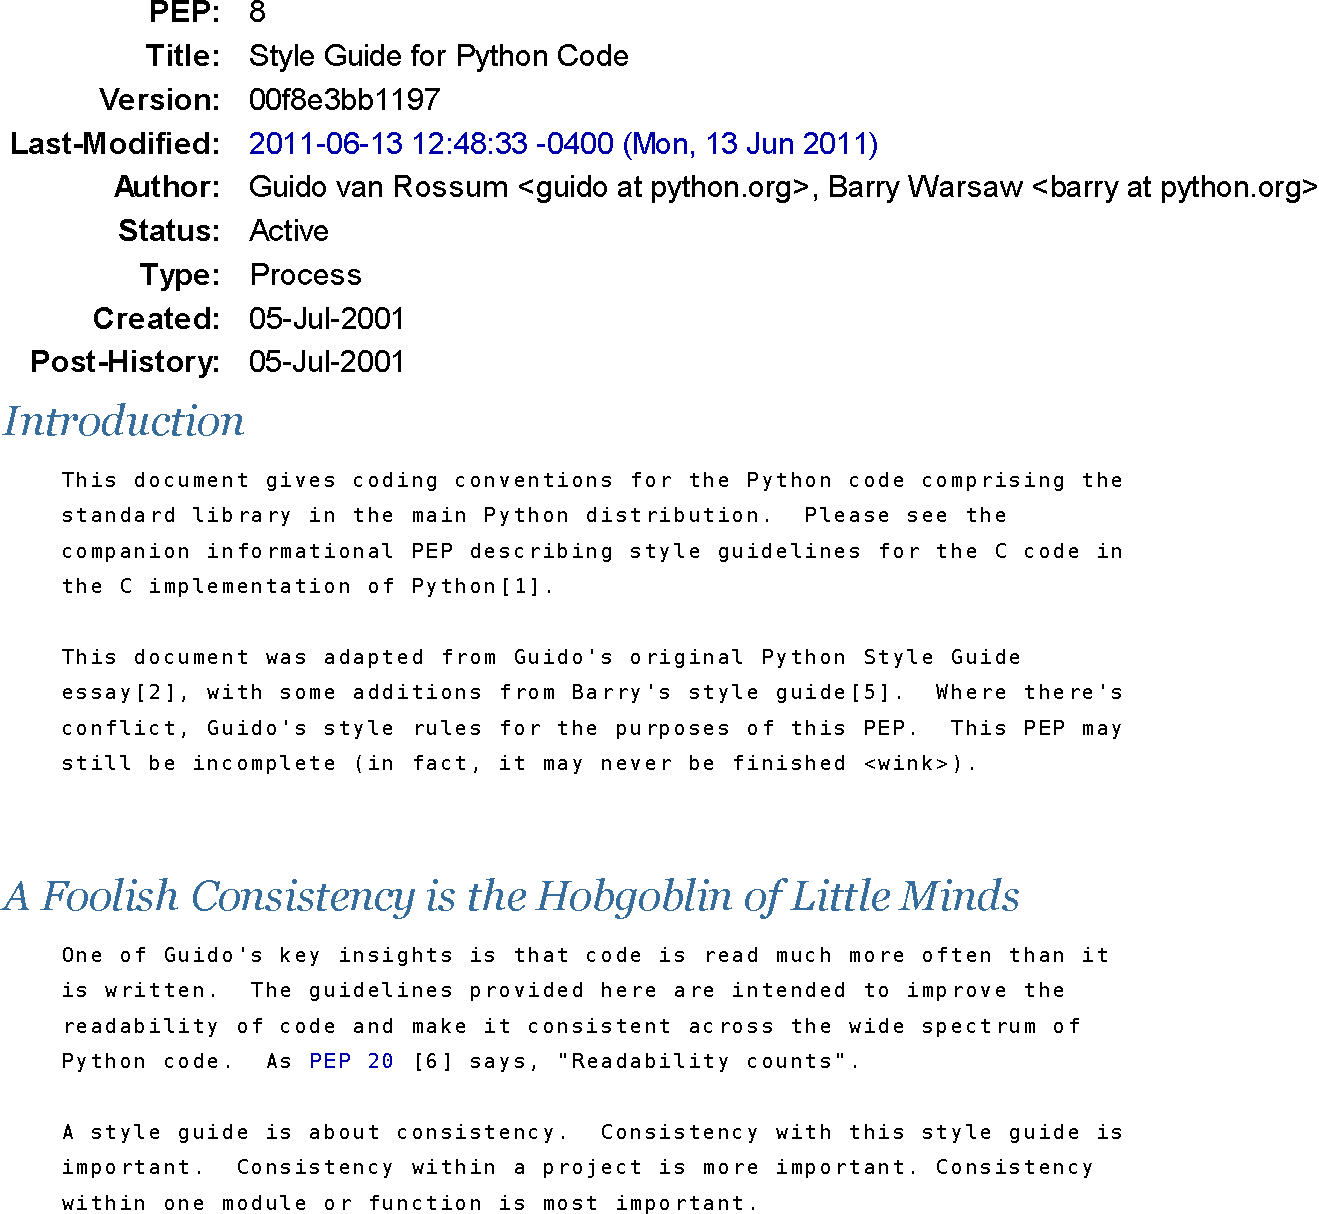
\includegraphics[width=0.9\textwidth]{python/pep8}
  \caption[Excerpt from \acl{PEP} 8]{Excerpt from \ac{PEP} 8: Style Guide for Python Code.}
\end{figure}

The Python project defines three types of \acp{PEP}.

\begin{enumerate}

  \item \spacedlowsmallcaps{Standards Track PEP} The most common form of \acp{PEP} describes a
    feature proposal for the Python language. They always consist of a design
    document and a reference implementation.

  \item \spacedlowsmallcaps{Informational PEP} Unlike the Standards Track PEP, this type of
    \ac{PEP} does not propose a new feature. It provides general guidelines or
    information about a certain issue of Python. However it does not
    necessarily reach consensus inside the Python community and so one is free
    to ignore Informational PEPs.

  \item \spacedlowsmallcaps{Process PEP} This kind of \ac{PEP} is quite like the Standards Track
    PEP, except that it applies to other areas than the Python language and
    describes processes around Python. For example any guidelines, decision
    making processes, development workflow and others are mostly Process PEPs.
    Additionally any \acp{PEP} which describe other \acp{PEP}, for example how
    a \ac{PEP} should look like, will be defined as a Process PEPs.

\end{enumerate}

The \ac{PEP} process begins with a feature proposal for Python. While all
bigger proposals require a \ac{PEP}, the Python project suggests to submit
small changes directly as a patch submission. A \ac{PEP} always has one or
several authors, who have the responsibility for it. They will begin by
submitting the \ac{PEP} to the Python project. More precisely it should be
presented to the \emph{python-ideas} mailing list and subsequently sent to the
\ac{PEP} editors. The \ac{PEP} editors will assign a number and a category as
mentioned above. Additionally, new \acp{PEP} always start with the \emph{Draft}
status. From there, the \ac{PEP} workflow begins.

\begin{figure}[htbp]
  \centering
  \begin{tikzpicture}[auto]
   \node[rectangle, rounded corners, draw=black, text width=6.5em, minimum height=2em, text centered]
     (draft) {Draft};
   \node[below=0.5cm of draft, rectangle, rounded corners, text width=6.5em, minimum height=2em, text centered]
     (dummy) {};
   \node[below=0.5cm of dummy, rectangle, rounded corners, draw=black, text width=6.5em, minimum height=2em, text centered]
     (deferred) {Deferred};

   \node[right=1cm of draft, rectangle, rounded corners, draw=black, text width=6.5em, minimum height=2em, text centered]
     (accepted) {Accepted};
   \node[below=0.5cm of accepted, rectangle, rounded corners, draw=black, text width=6.5em, minimum height=2em, text centered]
     (rejected) {Rejected};
   \node[below=0.5cm of rejected, rectangle, rounded corners, draw=black, text width=6.5em, minimum height=2em, text centered]
     (withdrawn) {Withdrawn};

   \node[right=1cm of accepted, rectangle, rounded corners, draw=black, text width=6.5em, minimum height=2em, text centered]
     (final) {Final};
   \node[below=0.5cm of final, rectangle, rounded corners, draw=black, text width=6.5em, minimum height=2em, text centered]
     (replaced) {Replaced};
   \node[below=0.5cm of replaced, rectangle, rounded corners, draw=black, text width=6.5em, minimum height=2em, text centered]
     (active) {Active};

   \draw[draw, -latex] ($(draft.south) - (1cm,0)$) -- ($(deferred.north) - (1cm,0)$);
   \draw[draw, -latex] ($(deferred.north) - (0.5cm,0)$) -- ($(draft.south) - (0.5cm,0)$);
   \path[draw, -latex] ($(draft.south) + (0.5cm,0)$) |- (rejected);
   \path[draw, -latex] (draft) |- ($(withdrawn.west) + (-0.5cm,0.8cm)$) |- (withdrawn.west);

   \draw[draw, -latex] (draft.east) -- (accepted.west);
   \draw[draw, -latex, dashed] (accepted.south) -- (rejected.north);

   \draw[draw, -latex] (accepted.east) -- (final.west);
   \draw[draw, -latex, dashed] (final.south) -- (replaced.north);
  \end{tikzpicture}
  \caption[Status Paths of \aclp{PEP}]{Possible paths of the status of \aclp{PEP}.}
\end{figure}

\paragraph{Draft}

This is the default state of any new \ac{PEP} on submission, as described
above.

\paragraph{Deferred}

A \ac{PEP} Editor can always, instead of assigning the Draft status, defer a
\ac{PEP}. Reasons for a deferral could be duplication, being poorly written,
lack of motivation by the author or not being in line with the Python
philosophy.

\paragraph{Accepted}

A \ac{PEP} will be able to get this status assigned, if all \ac{PEP} criteria
are matched. This includes a precise formulation of the \ac{PEP}, not breaking
backwards compatibility and finally be accepted by the \ac{BDFL}. However the
criteria are not fully binding and a \ac{PEP} just has to be accepted by the
\ac{BDFL}.

\paragraph{Rejected}

At this stage a \ac{PEP} can still be rejected. Mostly this status gets
assigned, if it turns out that the original idea did not fit the Python
project. The reject stage is just an option to drop a \ac{PEP}, after it was
accepted or not deferred.

\paragraph{Withdrawn}

A \ac{PEP} can also always be withdrawn by the author. This could help if an
author does not want to work on a \ac{PEP} anymore, for example because there
is a better solution available.

\paragraph{Final}

Once a \ac{PEP} has been accepted and has a reference implementation available,
it can get the status Final by the \ac{BDFL}.

\paragraph{Replaced}

Mostly for Informational PEPs, subsequent versions can replace a \ac{PEP}. In
this case the original \ac{PEP} would be marked as Replaced and superseded by
the new \ac{PEP}.

\paragraph{Active}

Informational and Process PEPs can also be marked as Active, if they will never
be completed. For example \ac{PEP} 1 \cite{Warsaw2000}, which describes the
process of \acp{PEP} has its status set to Active, as it is continually
improved and adapted to new workflows.

\begin{figure}[htbp]
  \centering
  \includegraphics[width=0.8\textwidth]{python/authors_by_month}
  \caption[Authors by Month, Python]
  {Amount of distinct authors of CPython over time. Python~2 seemed to provide
    a major reason for developers to join.}
\end{figure}

% }}}

% }}}


\section{PHP Project Analysis} % {{{

\marginnote{
\includegraphics[width=\marginparwidth]{php/logo}}

\noindent PHP is a server side, interpreted programming language designed for
web applications and development \cite{PHPIntro}. As such, it requires a web
server with a connected PHP installation. However it can also be used with a
command line interface. It is widely available for all major platforms and is
licensed under the PHP License \cite{PHPManual}. It is worth noticing, that
while it is a Free Software license, it is incompatible to the widely used
\ac{GPL}. PHP comes with an extensive standard library and supports many
programming paradigms, such as object oriented, imperative or procedural
programming styles. The abbreviation PHP originally stood for Personal Home
Page \cite{PHPHistory}. With PHP version 3, the project changed its name to PHP
Hypertext Processor. PHP is a very popular programming language for web
development and featuring a large number of websites
\cite{PHPW3Techs,PHPStats}.

\subsection{History} % {{{

In 1994, Rasmus Lerdorf created the first version of PHP for his own website,
naming the program Personal Home Page Tools \cite{PHPHistory}. He published the
bundle one year later, after rewriting the original version. That also included
the first name change to Forms Interpreter (\textsmaller{FI}) and then to
Personal Home Page Construction Kit the same year. At that time, PHP could be
considered as an advanced programming interface.

\begin{figure}[htbp]
  \centering
  \includegraphics[width=0.8\textwidth]{php/commits_by_author}
  \caption[Commits by Most Active Authors, PHP]
  {Monthly activity of the most active PHP developers. The climax of
    development in 2007 stalled and the most active developers appear to lose
    interest since then.}
  \label{fig:php:cba}
\end{figure}

However, it received another makeover in 1996, combining the two previous names
to PHP/FI. This time, PHP truly began to evolve to a full featured programming
language. It included several modules for database or browser interaction. This
version was also known as PHP/FI~2.0. Following a popularity boom in 1997 and
1998 it reached its limitations due to the design of the project and by being
almost solely developed by Lerdorf.

In 1997 Andi Gutmans and Zeev Suraski rewrote the PHP interpreter and
approached Lerdorf discussing the problems PHP had. Together, they rewrote and
redesigned the language and also changed the name to PHP Hypertext Processor.
Version 3.0 of PHP was then released in 1998 and replaced PHP/FI~2.0
completely. One of the most important features of the new approach was to
provide an interface for modules, which can be used directly from the
programming language.

The design of the language was changed further in 1998 improving performance
and the modularity of the codebase. The new engine was called Zend Engine and
provided the core of PHP~4.0, which was released in 2000.

Four years later, PHP~5 was released featuring the successor Zend Engine~2.0.
This release was incompatible to the previous 4.0 version and a large
initiative was planned and executed to promote the transition from PHP~4 to
PHP~5.

% }}}

\subsection{Community} % {{{

\begin{figure}[htbp]
  \centering
  \includegraphics[width=0.8\textwidth]{php/commits_by_year}
  \caption[Commits by Year, PHP]
  {Yearly overview of commits to PHP. The peaks could match with the
    development and releases of PHP~4.3 and PHP~5.}
  \label{fig:php:cby}
\end{figure}

The PHP project consists of a large user and developer community
\cite{Magnusson2010}. Additionally to the PHP interpreter, there are many
people working on PHP extensions and components, which get distributed
alongside the standard interpreter.

The PHP community provides a large amount of conferences and workshops to meet
in person and work together on PHP. While the \emph{International PHP
Conference} was the first of its kind in 2001 \cite{PHPConferences}, there are
many opportunities to meet other PHP contributors. A lot of local PHP User
Groups exist and provide weekly or monthly meetings and meet-ups such as
workshops.

Most of the communication inside the PHP project takes place through mailing
lists \cite{Magnusson2010}. There exist mailing lists for almost all aspects of
the project, however the most important is the \emph{internals} mailing list.
Most of the development process, future ideas and new contributions are handled
through that list. Of course, several \ac{IRC} channels and blogs of PHP
developers are also used.

Officially, there is no categorizing of developers and everyone is treated
equally. However the project uses a concept named \emph{karma}, which means
that one increases his karma by contributing to the project with code,
discussions and new ideas \cite{Magnusson2010}. Furthermore, several people are
responsible for different parts of the code or modules and can be classified
using those criteria \cite{PHPCredits}.

\paragraph{Developer}

One is called a PHP developer, once they get a PHP Subversion account.
According to the PHP community, an account needs to be earned, which means that
one has to provide several patches and contributions to the PHP project first.
Once one has shown enough commitment, they can apply for an account. The
account however will only be granted if a reference person approves.

\begin{figure}[htbp]
  \centering
  \includegraphics[width=\textwidth]{php/punchcard}
  \caption[Time Based View on Commits, PHP]
  {Time based view on commits of contributors. A lot of the commits appear to
    be happened during work days and times with some volunteer commits in the
    evenings and Sundays.}
  \label{fig:php:p}
\end{figure}

\paragraph{Module Author}

Each developer has the possibility to become a module author. This role has the
responsibility for a certain PHP module, which gets distributed with the PHP
release. Examples for such modules are database or imaging modules. For each
module, there can be more than one module authors, who share the
responsibility.

\paragraph{PHP Author}

This role defines a certain section of the PHP interpreter and its
responsibility for it. It is quite similar to the module author role, except
that it covers only PHP itself.

\paragraph{Language Designer}

Currently only Rasmus Lerdorf, Andi Gutmans and Zeev Suraski hold this role.
They are the only who can actively change the programming language syntax and
concepts.

% }}}

\subsection{Release Process} % {{{

\begin{figure}[bhtp]
  \centering
  \includegraphics[width=\textwidth]{php/releases}
  \caption[Major Releases of PHP]{Major releases of PHP.}
\end{figure}

In 2010, the PHP project set up a new release plan with detailed information
about how the release process should work \cite{PHPRelease}. Before,
individuals decided when a release happened and which features it included. The
new release cycle features two release managers who are voted by PHP
developers. The PHP project uses a versioning scheme with three numbers for
releases: major, minor and micro. Major releases get published quite seldom,
can break backwards compatibility and are planned a long time in advance. Minor
releases can have new features and bug fixes, however backwards compatibility
must be kept. Micro release are bug fix only releases where backwards and
\ac{API} compatibility must be kept. Each major release is followed by a number
of minor releases, which themselves are followed by a number of micro releases.

\begin{figure}[thbp]
  \centering
  \includegraphics[width=0.8\textwidth]{php/release_plan}
  \caption[Preliminary PHP Release Cycle]{Preliminary PHP release cycle.}
\end{figure}

Starting with PHP~5.4 a major or minor release will get published each year.
Each yearly release is then followed by a number of micro releases for two
years, which only contains bug fixes. After that period, only micro releases
with security relevant fixes will get published.

% }}}

\subsection{Development} % {{{

Most of the development process is handled through the PHP mailing lists
\cite{PHPRelease,Magnusson2010,PHPVoting}. Not every patch however needs to be
discussed and approved first, minor features or changes often get directly
committed to the repository. Every change needs to pass a peer review process,
where other developers review the made changes. As well every change gets
reviewed by other developers, who in case the need arises, discuss the change
on the developers mailing list. Generally the result is often a more
comprehensive change or new features.

To help the development and decision process, the PHP project keeps track of
new ideas, features and proposals through so called \ac{RFC} \cite{PHPRFC}.
Those are documents which describe the new feature and its rationale. A
\ac{RFC} document is always owned by at least one person, who is responsible
for it. The \ac{RFC} process begins with the author's submission of the
\ac{RFC} to the PHP wiki and an announcement to the \emph{internals} mailing
list. Depending on the importance and affected sections of the PHP project, the
following discussion period is set to a minimum of one to two weeks. It can be
longer however, but not shorter \cite{PHPVoting}.

\begin{figure}[thbp]
  \centering
  \includegraphics[width=0.8\textwidth]{php/commits_by_month}
  \caption[Commits by Month, PHP]
  {Amount of commits per month of core contributors. Even if the previous
    graphs showed a stalling development, the recent happenings in 2012 appear
    to show an again growing project.}
  \label{fig:php:cbm}
\end{figure}

After the discussion period has passed, the author can either call for a vote
or extend the discussion period as needed \cite{PHPVoting}. The vote is
announced on the mailing list and followed by a voting period which should be
at least one week, but can be extended if required.

Depending on the importance of a \ac{RFC}, it takes either 2/3 of all votes or
\unit[50]{\%} plus one to get accepted. The importance is defined by whether it
actually changes the syntax or behaviour of the PHP language and is therefore
irreversible or not. A failed proposal can be resurrected at earliest six
months after the last vote or if the author makes considerable changes to the
\ac{RFC}. There is no definition by the PHP project, what considerable changes
are, however the opinion is that it should be changed in a way, that it
significantly influences a vote's outcome.

All PHP developers are allowed to vote and, if needed, representatives from the
PHP community, such as participants of PHP related discussions or developers of
PHP appendant projects can participate in the voting process. Those however
have to be chosen by PHP developers \cite{PHPWhoVote}.

During the whole development process, a \ac{RFC} has an assignment status,
which can be one of the following \cite{PHPRFC}.

\paragraph{Draft}

Once a \ac{RFC} gets submitted to the PHP wiki, it gets this status assigned.
The Draft status means, that the \ac{RFC} is not ready yet for a discussion,
however it can be improved also by other people and a preliminary discussion
can be started.

\vfill
\begin{figure}[hbtp]
  \centering
  \begin{tikzpicture}[auto]
   \node[rectangle, rounded corners, draw=black, text width=6.5em, minimum height=2em, text centered]
     (draft) {Draft};
   \node[below=0.5cm of draft, rectangle, rounded corners, text width=6.5em, minimum height=2em, text centered]
     (dummy) {};
   \node[below=0.5cm of dummy, rectangle, rounded corners, draw=black, text width=6.5em, minimum height=2em, text centered]
     (withdrawn) {Withdrawn};

   \node[right=1cm of draft, rectangle, rounded corners, draw=black, text width=6.5em, minimum height=2em, text centered]
     (discussion) {Discussion};
   \node[below=0.5cm of discussion, rectangle, rounded corners, draw=black, text width=6.5em, minimum height=2em, text centered]
     (accepted) {Accepted};
   \node[below=0.5cm of accepted, rectangle, rounded corners, draw=black, text width=6.5em, minimum height=2em, text centered]
     (implemented) {Implemented};

   \node[right=1cm of discussion, rectangle, rounded corners, draw=black, text width=6.5em, minimum height=2em, text centered]
     (voting) {Voting};
   \node[below=0.5cm of voting, rectangle, rounded corners, draw=black, text width=6.5em, minimum height=2em, text centered]
     (declined) {Declined};

   \path[draw, -latex] (draft) -- (discussion);
   \path[draw, -latex] (discussion) -- (voting);
   \path[draw, -latex] ($(discussion.south) - (0.5cm,0)$) |-+(0,-0.2cm)-| (withdrawn);
   \path[draw, -latex] ($(voting.south) - (0.5cm,0)$) |-+(0,-0.2cm)-| (accepted);
   \path[draw, -latex] ($(voting.south) + (0.5cm,0)$) -- ($(declined.north) + (0.5cm,0)$);
   \path[draw, -latex] (accepted) -- (implemented);
   \path[draw, -latex] (declined.south) -- ++(0,-0.4cm) -- 
   ([yshift=-0.4cm, xshift=0.4cm] declined.south east) --
   ([yshift=0.4cm, xshift=0.4cm] voting.north east) -| (draft.north);
  \end{tikzpicture}
  \caption[Status Paths of PHP \acl{RFC}]
  {Possible paths of the status of \acl{RFC}.}
\end{figure}

\begin{figure}[htbp]
  \centering
  \includegraphics[width=0.8\textwidth]{php/authors_by_month}
  \caption[Authors by Month, PHP]
  {Amount of distinct authors of PHP over time. The number seems to be stable
    between 20 and 30 authors.}
  \label{fig:php:abm}
\end{figure}

\paragraph{Discussion}

Once the author of a \ac{RFC} announces it for discussion, it gets assigned to
this status. As previously described, the discussion phase starts with this
status.

\paragraph{Voting}

After the discussion phase the voting begins. While developers can vote for or
against the \ac{RFC}, the voting status gets assigned including a link to the
voting site.

\paragraph{Accepted}

Once a voting was successful, the \ac{RFC} is accepted and can be implemented.


\paragraph{Declined}

If the majority voted against the \ac{RFC}, it gets declined. After six months
and several changes to it, the author can resubmit it.

\paragraph{Implemented}

If the voting was successful, the \ac{RFC} will be implemented or taken into
action if it describes a community process.

\paragraph{Withdrawn}

The author can withdraw the \ac{RFC} without calling for a vote if they think
the \ac{RFC} is irrelevant or won't pass the voting.

% }}}

% }}}


\section{GNOME Project Analysis} % {{{

\marginnote{
\includegraphics[width=\marginparwidth]{gnome/logo}}

GNOME is a desktop environment for UNIX based systems. It is composed by a
collection of tools and programs including a desktop shell in order to provide
all the essential utilities a user might need when working with a computer.
Officially, GNOME is part of the \ac{GNU} project and licensed under the
\ac{GPL} and the \ac{LGPL}. The name GNOME was initially an acronym for
\emph{GNU Network Object Model Environment}, however that acronym was dropped.
The GNOME project targets ease of use and user friendliness and therefore aims
for coherent and good user interfaces \cite{GNOMEHIG}, accessibility,
internationalization, regular releases and good support for users and
developers. GNOME is a modular project, meaning that it consists of several so
called modules, which can be either applications, libraries or utilities. Since
the release of GNOME~3, the modules were reorganized into a GNOME core suite
and a GNOME apps suite. GNOME core provides everything to run a basic desktop
system and will therefore be analyzed in this context.

\begin{figure}[htbp]
  \centering
  \includegraphics[width=0.8\textwidth]{gnome/commits_by_author}
  \caption[Commits by most active authors, GNOME]
  {Monthly activity of the most active GNOME core developers. The
    disproportional amount of commits by Matthias Clasen can be interpreted
    with a high skill set and lots of effort he puts in the project.}
\end{figure}

\subsection{History} % {{{

GNOME was first announced and started in 1997 by Miguel de Icaza and Federico
Mena Quintero as a counterpart to KDE
\cite{German2003,GNOMEAbout,GNOMEAnnouncement}. Both were university students
at the time when they set their aim to produce a desktop environment using only
free software technologies. KDE relied on the Qt widget toolkit, which at the
time was licensed under a proprietary software license. Instead of using Qt,
they used the GTK+ toolkit originally developed for the GIMP graphics editor.
The GNOME project quickly grew into a large project which nowadays is the most
popular desktop environment for UNIX type operating systems. The desktop as
well as the developer technologies can be found on workstations and large
enterprises but also on mobile devices. With the recent GNOME~3 release a major
overhaul with a significant redesign of the desktop environment and an entirely
new user interface took place \cite{GNOMEPress}.

% }}}

\subsection{Community} % {{{

The GNOME project consists of a large user and developer community. While there
were about 3500 people contributing to GNOME and its applications, there is
also a big community around the project, which for example uses GNOME
technologies such as GStreamer or GTK+ \cite{GNOMEAbout,GNOMETeams}.

Most of the communication inside the project is handled through mailing lists
and \ac{IRC} channels. Almost every GNOME module has a dedicated mailing list
or \ac{IRC} channel. Global decisions are mostly handled through the
\emph{desktop-devel} mailing list. Additionally blogs are widely spread in the
GNOME community and contributors often write blog posts about achievements,
wishes or start discussions.

Next to several hackfests each year, the community holds a yearly conference
under the name \emph{GUADEC}. It stands for GNOME User and Developer European
Conference, and while the conference only took place in Europe so far it is
nevertheless considered worldwide \cite{GNOMEGUADEC}.

\begin{table}
  \centering
  \begin{tabularx}{\textwidth}{lXr}
    \toprule
    \tableheadline{Event}                   & \tableheadline{Venue}       & \tableheadline{Date} \\
    \midrule
    GUADEC \MakeUppercase{\romannumeral 1}  & Paris, France               & 2000 \\
    GUADEC \MakeUppercase{\romannumeral 2}  & Copenhagen, Denmark         & 2001 \\
    GUADEC \MakeUppercase{\romannumeral 3}  & Seville, Spain              & 2002 \\
    GUADEC \MakeUppercase{\romannumeral 4}  & Dublin, Ireland             & 2003 \\
    GUADEC \MakeUppercase{\romannumeral 5}  & Kristiansand, Norway        & 2004 \\
    GUADEC \MakeUppercase{\romannumeral 6}  & Stuttgart, Germany          & 2005 \\
    GUADEC \MakeUppercase{\romannumeral 7}  & Vilanova i la Geltrú, Spain & 2006 \\
    GUADEC \MakeUppercase{\romannumeral 8}  & Birmingham, England         & 2007 \\
    GUADEC \MakeUppercase{\romannumeral 9}  & Istanbul, Turkey            & 2008 \\
    Desktop Summit                          & Gran Canaria, Spain         & 2009 \\
    GUADEC \MakeUppercase{\romannumeral 10} & The Hague, Netherlands      & 2010 \\
    Desktop Summit                          & Berlin, Germany             & 2011 \\
    GUADEC \MakeUppercase{\romannumeral 11} & La Coruña, Spain            & 2012 \\
    \bottomrule
  \end{tabularx}
  \caption[Previous and planned GNOME conferences]{Previous and planned GNOME conferences.}
\end{table}

Due to the large and modular composition of the GNOME project, there are
similar roles for each module. Only very few teams and roles stand above all
modules. In this respect the developer community can be very much be seen as a
flat structure \cite{GNOMETeams,German2003,GNOMEDesignTeam,GNOMEReleaseTeam}.

\paragraph{Committer}

Any person who contributed a reasonable amount of improvements to the GNOME
project or to a single module can become a committer. A committer has full read
and write access to all GNOME repositories. Each commit will however be
reviewed and approved by the maintainer of the module. To get such an account,
one has to make a formal request to the Accounts Team along with one or several
vouchers who can confirm ones contributions to the GNOME project. Every module
maintainer or translation team leader can act as a voucher. Furthermore the
voucher will be responsible for the actions of the requesting person on the
repositories.

\paragraph{Maintainer}

Every module has one or more maintainers who will be responsible for releases,
reviewing patches and the direction of a module. They are the main contact for
the community and therefore act as the leader of a certain module. A single
module can be maintained by multiple maintainers and one maintainer can
maintain several modules. To become a maintainer one has either to create a new
module which gets incorporated into the GNOME project or be asked by another
maintainer.

\begin{figure}[htbp]
  \centering
  \includegraphics[width=0.8\textwidth]{gnome/commits_by_year}
  \caption[Commits by year, GNOME]
  {Yearly overview of commits to GNOME core. The leap in 2008 appears to be
    related to GNOME~2.22 or GNOME~2.24.}
\end{figure}

\paragraph{Release Team}

This team is responsible for a wide range of tasks concerning the development
process of the GNOME project. Their tasks include for example creating a
development schedule, making and publishing releases, approving or rejecting
freeze break requests and defining the module list for GNOME releases. The team
size is not fixed and can vary over time. Membership is only by invitation and
often only when one person leaves the team to free up one space. The leaving
person may recommend a new team member which the team will decide upon.

\paragraph{Design Team}

Since GNOME~3 the Design Team holds a much more important role in the GNOME
project as they primarily define the design of the GNOME user experience. This
is done by designing the user interface and workflow of GNOME modules.
Additionally they play an important part in the feature based development
process.

\paragraph{GNOME Founders}

Miguel de Icaza and Federico Mena Quintero, the original GNOME founders, played
an important role in the first years of the GNOME project. Nowadays however
they are more active in projects around GNOME technologies and often act as
visionaries.

\begin{figure}[h!tbp]
  \centering
  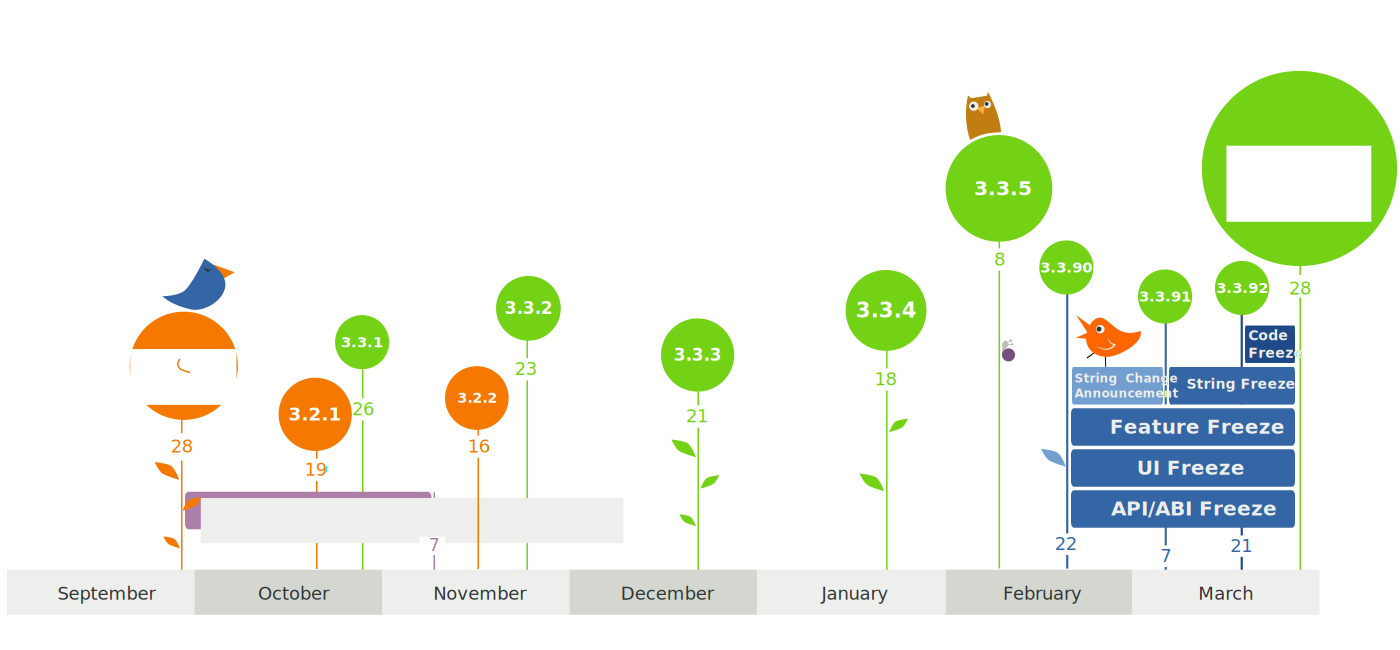
\includegraphics[width=0.95\textwidth]{gnome/gnome-timeline}
  \caption[GNOME 3.4 release schedule]{Release schedule which will lead to GNOME 3.4.}
\end{figure}

% }}}

\subsection{Release Process} % {{{

\begin{figure}[htbp]
  \centering
  \includegraphics[width=\textwidth]{gnome/releases}
  \caption[Major releases of GNOME]{Major releases of GNOME.}
\end{figure}

The GNOME project uses a version naming scheme with three numbers however
distinguishes only between major and minor releases
\cite{GNOMEDevelopmentSchedule,GNOMESchedule}. The numbers are however
nevertheless called major, minor and micro numbers. An incrementation of the
first number only occurs when the project does a ground-breaking change, such
as using GTK+2 for GNOME~2.x or the new user experience with the GNOME shell
and GTK+3 for GNOME~3.x. For the minor version number the GNOME project uses
odd numbers indicating an unstable series and even numbers for stable releases.
For example the unstable 3.1.x series will become the stable 3.2.x release
series.

The release schedule is fixed with a new major release appearing every six
months. To achieve this, the release team publishes a release schedule in the
same frequency \cite{GNOMEDevelopmentSchedule}. Over the years it stayed mostly
the same, while few minor changes may occur to comprise conferences or
holidays. The release schedule includes future stable minor releases, the two
schedules overlap.

Each stable release series consists of at least three releases which are named
with x.y.0 to x.y.2. Of course, a module maintainer can decide to provide more
stable releases \cite{GNOMEReleaseTeam}. The unstable series consists of eight
releases which are distributed over six months. The schedule furthermore
includes proposal and freeze periods which will be described in the following
\cite{GNOMEDevelopmentSchedule,GNOMESchedule}.

\begin{figure}[hbtp]
  \centering
  \includegraphics[width=\textwidth]{gnome/punchcard}
  \caption[Time based view on commits, GNOME]
  {Time based view on commits of Core contributors. It seems that most
    developers are employed. The high number on Monday can be explained with
    the release preparation which are always done on Monday evening.}
\end{figure}

\begin{figure}[htbp]
  \centering
  \includegraphics[width=0.8\textwidth]{gnome/commits_by_month}
  \caption[Commits by month, GNOME]
  {Amount of commits per month of Core contributors. The project quite shows a
    linear growth with peaks every six months.}
\end{figure}

\paragraph{Feature proposal period}

After a major release gets published the feature proposal period starts. GNOME
developers can propose features for the next major release and discuss them
with the community. Approximately a month later, when the first unstable
release gets published, the proposal period ends. Around two weeks later the
release team meets and decides about proposed features with the community input
given up to this point.

\paragraph{The Freeze}

With the release of the first beta the first freeze takes action. No user
interface changes, new features or developer \ac{API} changes are allowed
without approval from the release team. This excludes of course bug fixes.
Additionally new translatable strings must be announced to the translation and
documentation team.

\paragraph{String Freeze}

With the second beta release no string changes are allowed anymore without
confirmation of both the release and translation team.

\paragraph{Hard Code Freeze}

With the release of the release candidate no source code changes are allowed
without approval of the release team. Documentation and translation however can
continue. After publishing the next major GNOME release the Hard Code Freeze
ends but all other freezes remain in action for the stable series.

\begin{figure}[htbp]
  \centering
  \includegraphics[width=0.8\textwidth]{gnome/authors_by_month}
  \caption[Authors by month, GNOME]
  {Amount of distinct authors of GNOME core over time. Especially the
    development of GNOME~3 which started in 2010 appears to have attracted
    additional developers.}
\end{figure}

% }}}

\subsection{Development} % {{{

Before the release of GNOME~3, the release team together with the community
decide about the inclusion of new modules. The development of each module was
planned and executed by the maintainers. Since GNOME~3, the development
workflow changed into a more design driven development approach. This means
that all new features concerning user interfaces or applications have to go
through the design team \cite{GNOMEDesignTeam}. This leads to a consistent
process with a uniform user interface. However the design team has no decision
making authority and a maintainer can ignore the design team's proposal.

Next to the design driven approach the module inclusion changed to a feature
inclusion approach \cite{GNOMEFeatures3.4,GNOMERoadMap}. Every GNOME
contributor can create a feature proposal in which one describes a feature they
would like to see in the next stable GNOME release. A feature proposal is
composed by a description of the problem which will be solved, one or more
authors, a list of involved parties and the current state of the proposal. All
of these fields are required and a feature will not be accepted until all are
completed. After each major release and until about a month later, one can
propose a feature for inclusion. The community has time to discuss the features
and improve them for roughly one and a half months. After that time the release
team will meet and depending on the feedback of the community decide about the
inclusion of each feature. If a feature gets accepted the author of the feature
will be its leader and responsible for the completion. With the release of the
first beta release and the establishment of the Feature, \ac{UI} and
\ac{API}/\ac{ABI} Freeze the feature has to be finished and working. If not, it
may be postponed to the next major release.

% }}}

% }}}


\section{KDE Project Analysis} % {{{

\marginnote{\centering
\includegraphics[width=0.5\marginparwidth]{kde/logo}}

KDE is a desktop environment designed to run on UNIX based systems as well as
Microsoft Windows and Mac \textsmaller{OS X} systems \cite{KDEPress,KDEAbout}.
Since 2010 and the release of KDE~4.4 the project is known as \ac{KDE SC}. It
is composed by the desktop environment named Plasma Desktop and several core
applications for the daily needs. \ac{KDE SC} is licensed under the \ac{GPL}
and \ac{LGPL}. The name was originally an acronym for Kool Desktop Environment
and later for K Desktop Environment, however it is no longer in use. KDE is a
modular project consisting of several libraries which allow developers to build
their programs around the platform. As the KDE project and the \ac{KDE SC}
stand for a wide range of technologies and applications, this analysis will be
limited to the core of the \ac{KDE SC}, also known as KDE Base.

\subsection{History} % {{{

KDE was first announced by Matthias Ettrich in 1996 as a desktop
environment for end users with the same look and feel for all applications
\cite{KDEAnnouncement}. The name KDE was a word play with the existing
Common Desktop Environment (CDE), which was highly popular at that time. Matthias Ettrich chose the Qt framework as the graphical library, which was and is
developed by the company Trolltech. KDE~1.0 was then released in 1998
\cite{KDEHistory}. At the same time, Trolltech dual licensed the framework
under the Q Public License (QPL) and a proprietary software license. However,
it was debated if that license was compatible with the \ac{GPL} and in 2000 the
framework was licensed under the \ac{GPL} which ceased the criticism.

In 2009 the KDE project renamed the project to \ac{KDE SC} and redefined the
project as a community which delivers free software for user interfaces by
emphasizing the KDE technologies \cite{KDESC}. All software created with KDE
technologies are KDE projects. However \ac{KDE SC} only contains projects which
derive from the project itself and share a common release cycle.

\ac{KDE SC}~4 was a new approach to the desktop metaphor and created a new user
experience for users. The centerpiece is the Plasma Workspace which exists for
several devices, such as for desktop computers, netbooks, tablets and
smartphones.

% }}}

\subsection{Community} % {{{

The KDE project is one of the largest \ac{FOSS} projects and according to the
community the second largest after the Linux Kernel \cite{KDEPress}. There are
about 1800 active contributors to the project and its surroundings and is used
by over a million people. Also, the community spans around projects based on
KDE technologies.

Most of the communication in the KDE project takes place via mailing lists,
most importantly \emph{kde-devel} and \emph{kde-core-devel}
\cite{KDEProjectManagement,KDEContribute}. While the first one is mostly used
for communication by application developers, the latter one is for
communication on the KDE core project. Furthermore communication can happen
over \ac{IRC} channels, blogs or forums.

The most important KDE conference is the annual \emph{Akademy} which is held at
different locations in Europe \cite{KDEHistory}. The first KDE conferences were
however named after the current release which started with \emph{KDE One} in
1997. That is also the reason, why the conferences did not take place annually
at that time. In 2004 it changed the name to Akademy. Beginning with 2009 the
project incorporated the conference into the \emph{Desktop Summit} in
collaboration with the GNOME project.

\begin{table}
  \centering
  \begin{tabularx}{\textwidth}{lXr}
    \toprule
    \tableheadline{Event}   & \tableheadline{Venue}           & \tableheadline{Date} \\
    \midrule
    KDE One                 & Arnsberg, Germany               & 1997 \\
    KDE Two                 & Erlangen, Germany               & 1999 \\
    KDE Three Beta          & Trysil, Norway                  & 2000 \\
    KDE Three               & Nürnberg, Germany               & 2002 \\
    Kastle                  & Nové Hrady, Czech Republic      & 2003 \\
    aKademy                 & Ludwigsburg, Germany            & 2004 \\
    aKademy                 & Málaga, Spain                   & 2005 \\
    aKademy                 & Dublin, Ireland                 & 2006 \\
    aKademy                 & Glasgow, Scotland               & 2007 \\
    Akademy                 & Sint-Katelijne-Waver, Belgium   & 2008 \\
    Desktop Summit          & Gran Canaria, Spain             & 2009 \\
    Akademy                 & Tampere, Finland                & 2010 \\
    Desktop Summit          & Berlin, Germany                 & 2011 \\
    Akademy                 & Tallinn, Estonia                & 2012 \\
    \bottomrule
  \end{tabularx}
  \caption[Previous and Planned KDE Conferences]{Previous and planned KDE conferences.}
\end{table}

\begin{figure}[htbp]
  \centering
  \includegraphics[width=0.8\textwidth]{kde/commits_by_author}
  \caption[Commits by Most Active Authors, KDE]
  {Monthly activity of the most active KDE core developers. The most active
    developers almost switched completely when comparing the inception phase to
    nowadays.}
\end{figure}

Due to the size of the KDE project it is organized around many independent
teams with a communication structure between them. There are few groups who
stand above those teams and only take care about coordinating the project
\cite{KDEDevelopmentModel,KDEProjectManagement}.

\paragraph{Contributor}

After having contributed to any KDE project for some time and planning to
contribute in the future, a KDE Contributor account can be requested
\cite{KDEContribute,KDEContributor}. In the request one must state why one is
interested in having an account. The KDE sysadmin team will then check the
application and grant an account or not.

\paragraph{Module Coordinator}

As the KDE project is highly modular, each application or library has an
independent team with its own structure besides a few exceptions. A module
coordinator plans and executes releases and the direction of a single module.
As the teams are so diverse, there are many ways to become a module
coordinator. The most obvious is of course by unweary contributions to a
project.

\begin{figure}[htbp]
  \centering
  \includegraphics[width=0.8\textwidth]{kde/commits_by_year}
  \caption[Commits by Year, KDE]
  {Yearly overview of commits to KDE base. The development and release of KDE~4
    and following releases in 2008 certainly attracted a lot of attention.}
\end{figure}

\paragraph{Core Team}

One of the most important teams is the Core Team as it defines the overall
direction the project is heading \cite{KDEProjectManagement}. There is no
single person inside the team responsible for decision making, instead the team
discusses the issue and comes up with a solution together. The primary
communication method is the \emph{kde-core-devel} mailing list which is
publicly readable, however an approval is required to join it. The KDE project
does not define clear restrictions to membership and therefore a membership is
granted by invite only after distinguishing or outstanding work for the KDE
project.

\paragraph{Release Team}

The actual release and the release schedules are provided and enforced by the
Release Team \cite{KDEReleaseTeam}. It is composed by module coordinators and
other release team members who actually implement the releases. The Release
Team makes sure that all modules are following the release schedule and are in
a good shape. Also they decide on code freeze breaks and take decision about
future features of a release.

\paragraph{KDE Founder}

Matthias Ettrich, the founder of the KDE project is no longer actively involved
in the project as he works full time on the underlying Qt framework. However he
has still an important voice in the community and contributes indirectly to KDE
by his role in the Qt project.

% }}}

\subsection{Release Process} % {{{

\begin{figure}[htbp]
  \centering
  \includegraphics[width=\textwidth]{kde/releases}
  \caption[Major Releases of KDE]{Platform and standard releases of KDE.}
\end{figure}

The KDE project uses a versioning scheme with three numbers and distinguishes
between major and minor releases
\cite{KDEReleaseTeam,KDEReleaseSchedule,KDESchedule}. The numbers are called
major, minor and micro numbers. The major and minor numbers define major
releases while the micro number defines maintenance releases. The release is a
platform or standard release depending on whether the major or minor numbers
change. A platform release defines a new series of releases which can break
backwards compatibility to the previous platform release. They are often
planned a long time ahead, usually including changes of used libraries or used
versions switches. A standard release however has to maintain backwards
compatibility with its series. They can have new features and user interface
changes, however a KDE application has to work on all releases of the same
platform. Maintenance releases are not allowed to come with new features,
except bug fixes or small enhancements. Beginning with \ac{KDE SC}~4 the cycle
changed to a major release every six months and a maintenance release roughly
every month except when a major release comes out.

To ensure the release schedule, the release team publishes a new release
schedule after each major release. The schedule includes all deadlines and
freezes which will lead to the next major release and includes future
maintenance releases. This means of course that two release schedules will
overlap during the month before the new major release. The following freezes
and releases are provided and enforced by the release team
\cite{KDEReleaseSchedule}.

\paragraph{Soft Feature Freeze}

Approximately three weeks before the first beta release no new features are
allowed except already approved and planned features. Not finalized features
have to be postponed to the next major release.

\begin{figure}[hbtp]
  \centering
  \includegraphics[width=\textwidth]{kde/punchcard}
  \caption[Time Based View on Commits, KDE]
  {Time based view on commits of Core contributors. The times are almost
    equally distributed probably meaning that there exist a lot of employed and
    volunteering developers in the community.}
\end{figure}

\begin{figure}[htbp]
  \centering
  \includegraphics[width=0.8\textwidth]{kde/commits_by_month}
  \caption[Commits by Month, KDE]
  {Amount of commits per month of Core contributors. Again, the development
    phase of KDE~4 and following releases is quite visible.}
\end{figure}

\paragraph{Dependency Freeze}

Approximately two weeks before the first beta release no new or additional
dependency versions are allowed anymore. However it is possible to request an
exception by the release team.

\paragraph{Soft Message, Soft API and Hard Feature Freeze}

One week before the first beta release no new strings and changes to the
existing messages can be made except corrections. Additionally the existing
\ac{API} should be almost finished and if changes are made they should be
reported to the relevant teams. Lastly no new features can be added to the
projects, even if they were planned for this release cycle.

\paragraph{Beta Release}

Approximately two months before the major release the first beta release gets
published. This is usually followed by a second beta release two weeks later.

\paragraph{Hard API, Message and Documentation Freeze}

Five weeks before the major release the \ac{API}, translatable messages and the
documentation must be finished and can't be changed anymore.

\paragraph{Release Candidate}

Approximately a month before the final release the first release candidate will
be published. Two weeks later the second release candidate follows.

\begin{figure}[htbp]
  \centering
  \includegraphics[width=0.8\textwidth]{kde/authors_by_month}
  \caption[Authors by Month, KDE]
  {Amount of distinct authors of KDE base over time. The project appears to
    grow quite linearly with a small down before the start of the KDE~4
    development and the appropriate boost during and after the development.}
\end{figure}

\paragraph{Final Release}

The final release will then be published three weeks after the last release
candidate.

\paragraph{Minor Releases}

A new minor release will be published each following month until the next major
release gets published. This normally leads to four minor releases.

% }}}

\subsection{Development} % {{{

During the development of a new major release, new project goals are set using
feature proposals \cite{KDEDevelopmentModel,KDEFAQ}. This normally happens
after each major release when KDE developers have the time to propose new
features for the next major release. Each feature must have an author who is
willing to implement it. This often limits the number of features to already
contributing KDE developers. A KDE developer is free to implement the feature
by himself, however the process is often accompanied by a discussion with the
specific team and several adjustments to the implementation.

During the soft feature freeze is decided whether the feature will be available
for the upcoming major release or if it will be postponed to the next major
release. If the implementation already started and is almost finished, it can
continue. Otherwise it will be postponed. This development process is a quite
deliberate approach where people are free to implement what they see missing in
the project.

% }}}

% }}}


\section{Proposition for a Project Analysis Catalogue} % {{{

To characterize the development processes of \ac{FOSS} projects, the following
catalogue was established based on the previous gathered data and analysis. By
covering all listed points one a project should have been analyzed thoroughly
and lead to a reasonable breakdown of all projects.

\subsection{Description of the Project}

A general description about the project should be provided to inform about the
goals and current state of a project. They are essential to put a project under
the right light and make it comparable with similar projects.

\subsection{Project Category}

In order to provide methods to compare projects, the project category can help
to contrast projects of the same and other categories. As such it doesn't
provide too much information about the project itself, but is useful for later
comparisons with other projects.

\subsection{Scope of Analysis}

As \ac{FOSS} projects often are hard to analyze due to their size and unclear
definition of modules, the scope will be limited to a well known subset of the
whole project. This helps to provide a thorough analysis without leaving things
unattended.

\subsection{License}

Without being licensed under a \ac{FOSS} license, a project cannot be counted
as a \ac{FOSS} project. Listing all used licenses can ensure this fact. However
it is also interesting to see whether development models and communities differ
if they are using a different \ac{FOSS} license.

\subsection{History}

A project's history shaped the community and the structure of a project to the
state it can be found today. As such the analysis of the history can bring up
interesting findings.

\paragraph{Founders}

In some projects, the original founders are still present and have a
influential voice, in others the original authors are no longer involved. To
analyze this further, the authors have to be introduced and their role will be
analyzed in the community part.

\paragraph{Project Age}

Projects always need time to evolve and to find their best development process.
As this needs time, the project age can give some information in what
development process state this project is and how it will evolve in the future.

\subsection{Community}

The people behind the project are the driving force. Without them, a project
would not exist. Therefore it is important to analyze the diverse community of
a project.

\paragraph{Size of the Community}

An important measure is the approximate size of a community. Several structural
decisions and changes inside the project can depend on this size.

\paragraph{Communication inside the Project}

The communication is a vital thing in an open project. It is interesting to
compare the different methods of communication in several projects depending on
their development structure and size.

\paragraph{Conferences and Meet-ups}

Meetings of developers are an important element of the development process in
\ac{FOSS} projects. It also shows, that there is enough interest available to
provide the money needed for preparing such events.

\paragraph{Roles}

The development process is often defined and lead by important roles in the
project. Also, depending on what role a person has in the project, his
influence varies.

\paragraph{Role of the Founders}

In some projects the founders are still actively involved and in some not.
Depending on that, the founders often have a very important role in the project
development process.

\subsection{Release Process}

The release process is the action which leads to new releases. As this is a
very essential part of the development processes it will be analyzed with the
following classification.

\paragraph{Version Naming}

Each project provides a specific version naming scheme to which they adopt and
which characterizes major, minor or bug fixing releases. This information is
vital to understand the project's release schedule.

\paragraph{Characterization of Major and Minor Releases}

Most projects provide some kind of major and minor releases where major
releases do come with new features often backwards incompatible changes. Minor
releases on the other hand often only contain fixes. It is now interesting to
see where and how the line between the two is drawn.

\paragraph{Release Schedule}

The release schedule defines the concrete plan up to a new release and is often
either time or causal dependent. As they define deadlines or important steps in
the process of creating new releases it is most interesting to compare
different schedules.

\paragraph{Important Steps in the Schedule}

These often define freezes or specific points in time when all members of the
project are restricted to for example not provide new code in order to increase
the stability of the new release.

\subsection{Development}

The actual development is closely interweaved with the release process and
defines how and when the development of a project takes place.

\paragraph{Development Lead}

It is hardly imaginable that there exist projects which have a completely
unstructured development process and have no development leaders in place. This
point covers, if existent, groups of people who define new features and lead
the development process.

\paragraph{Development Workflow}

The actual development process as often defined by the project leaders provides
ways and methods to propose and develop new features for the upcoming release.
It also covers the daily development and how new code finds it's way into the
project's repositories.

\paragraph{Feature Inclusion Process}

In some way features find their way into a project. Whether projects do have
established a concrete process for how and when new features come into a
project or not will be capped in this point.

% }}}

\section{PostgreSQL Project Analysis} % {{{

\marginnote{
\includegraphics[width=\marginparwidth]{postgresql/logo}}

The PostgreSQL project provides an \ac{ORDBMS} which runs on all major systems
such as Linux, UNIX, Microsoft Windows or Mac OS X
\cite{PostgreSQLAbout,PostgreSQLFAQ}. The group behind the project is known as
PostgreSQL Global Development Group which consists of several volunteers and
employed developers. PostgreSQL is quite popular amongst it's users and has won
several prizes for the best database management system \cite{PostgreSQLAwards}.
According to the project it is the leading \ac{FOSS} database system with
thousands of users and contributors \cite{PostgreSQLPressKit}.

\subsection{Project Category}

PostgreSQL is a database management system, more specifically a \ac{ORDBMS}
\cite{PostgreSQLAbout}.

\subsection{Scope of Analysis}

The PostgreSQL Core Distribution will be analyzed, which consists of the
PostgreSQL database server, several tools and bindings around it
\cite{PostgreSQLDownload}.

\subsection{License}

The PostgreSQL project makes use of the PostgreSQL license, which is a
\ac{FOSS} license \cite{PostgreSQLFAQ,PostgreSQLLicense}. It only requires to
maintain the copyright and licensing information in the licensed source code
and therefore it is quite similar to a BSD license.

\subsection{History}

The project was started in 1986 by Lawrence A. Rowe and Michael R. Stonebraker
at the University of California in Berkeley under the name POSTGRES
\cite{PostgreSQLHistory}. Not until 1996 it was developed in a university style
fashion trying to explore new areas in database management systems. It was then
released as \ac{FOSS} by two students of Stonebraker with the new name
PostgreSQL the adopted \ac{SQL}. It then received a big development boost and
emerged to one of the leading \acp{ORDBMS}.

\subsection{Community}

The PostgreSQL project has a quite large community available which will be
described in the following.

\paragraph{Size of the Community}

According to the project there are 6 core team members, 38 major contributors
and 42 contributors \cite{PostgreSQLContributors}. Adding no longer active
persons the number sums up to around 140. The number of total contributors
might however be higher, as the project only includes people who have made
contributions over a long time.

\paragraph{Communication inside the Project}

The communication mostly happens over mailing lists, although also \ac{IRC}
channels exist. The most important mailing list for development is the
\emph{pgsql-hackers} mailing list \cite{PostgreSQLDevFAQ}.

\paragraph{Conferences and Meet-ups}

The most important international conference is the annual \emph{PgCon} which
first happened in 2007 \cite{PostgreSQLEvents}. However there are a lot of
local conferences and workshops available.

\paragraph{Roles}

The developers are split into three groups \cite{PostgreSQLContributors}. The
core team decides on the general direction of the PostgreSQL project as well as
the release cycle and the releases. Major contributors are people who
introduced or maintain big features to the project. The contributors are all
other who provide patches to the project.

\paragraph{Role of the Founders}

Michael R. Stonebraker and Lawrence A. Rowe did not follow the project when it
was published as \ac{FOSS} in 1996 \cite{PostgreSQLHistory}. They are therefore
no longer actively involved in the project.

\subsection{Release Process}

The used release process is highly structured and will be described in the
following.

\paragraph{Version Naming}

The PostgreSQL project uses a three digit number scheme which consists of a
major, minor and micro number \cite{PostgreSQLVersioning}.

\paragraph{Characterization of Major and Minor Releases}

The incrementation of a major or minor number defines a major release including
new features and often backwards incompatible changes
\cite{PostgreSQLVersioning}. Such a release occurs roughly once a year
\cite{PostgreSQLDevelopment,PostgreSQLFAQ}. For each major release there exist
a number of minor releases which are defined by incrementing the micro version
number. Only bug and security fixes are allowed for those releases. Each major
release is supported for five years by the PostgreSQL project. However in some
cases the project can decide to drop support for a specific release if bugs
cannot be resolved without risking the stability.

\paragraph{Release Schedule}

As major releases occur every year, the project uses the same release schedule
every year along with some minor improvements from the last years
\cite{PostgreSQLDevelopment}. The release schedule gets planned and decided
during the PgCon conference. It basically starts each June with a commit review
in which possible patches might be included in the next major release. Such
reviews, also known as Commit Fest happen four times each two months apart. In
the month between an alpha release is published. After the last Commit Fest,
more alpha releases can follow, if not beta releases are published. If no more
critical errors are found several release candidates will be published which
will lead to the next major release.

\paragraph{Important Steps in the Schedule}

The Commit Fest are the only possibility to add new features to the project and
are therefore a vital part of the development process
\cite{PostgreSQLDevelopment,PostgreSQLCommitFest}. 

\subsection{Development}

The development of the PostgreSQL project is closely entangled with the release
process and will be described in the following.

\paragraph{Development Lead}

The PostgreSQL project is mostly driven by the core team
\cite{PostgreSQLDevFAQ,PostgreSQLFAQ,PostgreSQLContributors}. Quite all
decisions are made by them as well as most new features and code contributions.

\paragraph{Development Workflow}

Small patches are often submitted directly to the repository if they are done
by a major contributor or a core team member \cite{PostgreSQLDevFAQ}. All other
patches however have to be reviewed and therefore be sent to the pgsql-hackers
mailing list. New features are proposed in the Commit Fests.

\paragraph{Feature Inclusion Process}

The already mentioned Commit Fest is a periodic break in which no new
development is done, however already existing patches are reviewed and get
feedback \cite{PostgreSQLCommitFest}. Not only the core team does those reviews
but also other developers. A single Commit Fest usually runs for about one
month explaining the gap of one month between each Commit Fest. One such event
is lead by a Commit Fest Manager who is responsible that all submitted patches
will be reviewed. Often, a review results in a discussion on the mailing list
and follows an acceptance, a return with feedback or a rejection. A patch can
have several states, depending on whether it is in progress or if it is
finished \cite{PostgreSQLCommitFestRunning}. If a patch is in progress, the
following states might apply.

\begin{description}

  \item[Needs Review] A patch is not reviewed and waiting for a review.

  \item[Waiting on Author] A new version of the patch is expected by the
    author.

  \item[Discussing Review Results] The review was done, however it is
    discussed on the mailing list.

  \item[Ready for Committer] The review was done and no issues were
    found. It is now waiting for a final review.

\end{description}

\noindent The in progress states of a patch are the following.

\begin{description}

  \item[Returned With Feedback] The patch was reviewed and feedback was
    given. A new version of the patch is expected for the next Commit Fest.

  \item[Rejected] The patch was rejected and won't make it into the next
    major release.

  \item[Committed] The patch was applied and no remaining issues are
    assured.

\end{description}

% }}}

\section{MySQL/MariaDB Project Analysis} % {{{

\marginnote{
\includegraphics[width=\marginparwidth]{mariadb/logo}}

MySQL is according to the project the world's most used \ac{ORDBMS}
\cite{MySQLSun}. It runs on all major platforms and is widely used for many web
applications. MySQL was originally developed by MySQL AB, later bought by Sun
Microsystems and now owned by Oracle Corporation
\cite{MySQLSun,MySQLOracle,MySQLHistory}.

MariaDB was forked from the original MySQL when Oracle bought Sun Corporations
as it was unclear how the development and licensing of MySQL would change after
Oracle's acquisition \cite{MySQLAbout,MySQLBehind}. It is intended to be a
\emph{drop-in} replacement for MySQL with full compatibility to it. Also, many
of the original MySQL developers moved to the MariaDB project making it
interesting to analyze both projects together.

\subsection{Project Category}

MySQL and MariaDB are database management systems, more specifically
\acp{ORDBMS} \cite{MySQLAbout}.

\subsection{Scope of Analysis}

The MySQL Server package and MariaDB will be analyzed. Both provide a
compatible database server together with several tools for running it.

\subsection{License}

MySQL is dual-licensed under the \ac{GPL} and a proprietary license. MariaDB is
single licensed under the \ac{GPL} \cite{MySQLLicense}.

\subsection{History}

The MySQL project was started in 1994 by Michael Widenius and David Axmark by
lanching the company MySQL AB \cite{MySQLHistory}. Originally it was a clone of
the at that time quite popular mSQL project. In 2000 MySQL was released as
\ac{FOSS} under a dual licensing model. Sun Microsystems bought MySQL AB in
2008 which lead to the abandonment of the MySQL founders Micheal Widenius and
David Axmark \cite{MySQLSun}. In 2010 Oracle Corporation bought Sun
Microsystems and announced changes to the current development processes
\cite{MySQLOracle}. As the future of MySQL in terms of \ac{FOSS} was quite
unclear at that time Michael Widenius forked MySQL in order to provide a
community developed, \ac{FOSS} database \cite{MySQLBehind}. The first version
of MariaDB was released in 2010 as MariaDB 5.1 which is compatible to MySQL 5.1
\cite{MySQLMariaDB5.1}. Since then the MariaDB project tries to stay compatible
with MySQL but also to provide better performance and more features.

\subsection{Community}

As most of the key-authors of MySQL moved to different projects, such as
MariaDB and as there is not much insight available about the current happenings
inside Oracle, the MariaDB community will be analyzed including facts about the
pre Oracle era of MySQL.

\paragraph{Size of the Community}

The specific size of the community is not known, however it is fracturing after
the two acquisitions by Sun Microsystems and Oracle Corporation. The newly
founded Monty Program Ab company however lists at least 20 people working on
MariaDB \cite{MySQLBehind}.

\paragraph{Communication inside the Project}

The communication mostly happens over mailing lists, although also \ac{IRC}
channels exist. The most important mailing list for development are the
\emph{maria-developers} and \emph{maria-captains} mailing lists
\cite{MySQLDevelopers}.

\paragraph{Conferences and Meet-ups}

The MariaDB project has not yet set up a conference, however the MySQL project
mostly meet at the yearly \emph{MySQL Users Conference \& Expo} which first
happened in 2003 \cite{MySQLConference}.

\paragraph{Roles}

The developers are split into two groups. A developer is a person who produces
enhancements and new features for MariaDB
\cite{MySQLContributingCode,MySQLContributing,MySQLCaptain}. However he has no
right to commit his work which has to be reviewed. The captains are developers
who are working for a long time for the project and have made substantial
improvements. To become a captain one has to make a formal request on which the
other captains will vote \cite{MySQLCaptain}. Captains give the direction of
the project, do the code reviews and take care of the project. Finally there
exists a Release Coordinator which normally is a captain
\cite{MySQLReleaseCoordinator}. By definition he gains no additional rights and
only leads the communication and release management of the project.

\paragraph{Role of the Founders}

Micheal Widenius took a vital role in the fork and new project MariaDB
\cite{MySQLBehind,MySQLAbout}. If nevertheless MariaDB is mostly driven by
MariaDB captains (which he belongs too) he has an important voice in the
community and still gives general directions. David Axmark however left Sun in
2008 and is not really actively involved in either the MySQL nor MariaDB
project however follows their development.

\subsection{Release Process}

The used release process is structured and will be described in the following.

\paragraph{Version Naming}

The MySQL/MariaDB project uses a three digit number scheme which consists of a
major, minor and micro number \cite{MySQLVersion}.

\paragraph{Characterization of Major and Minor Releases}

The incrementation of a major number defines big and often incompatible changes
to their predecessors \cite{MySQLVersion}. In the current releases it marks the
file format in which the database is stored. A major release is defined by an
incrementation of the minor number and allows new features to be added to the
release. In most cases the releases are backwards compatible, but if not, there
are always upgrade paths available \cite{MySQLMariaDB5.1}. Finally, the micro
number defines minor releases in which only bug and security fixes may apply.

\paragraph{Release Schedule}

The MariaDB project does not have a fixed release schedule and is quite similar
to the MySQL release schedule
\cite{MySQLReleaseCriteria,MySQLRoadmap,MySQLPlans}. It has criteria in place
when specific releases can happen. After the last stable major release, all new
features for the next stable major release will be collected. Every feature a
MariaDB developer agrees to implement in the timeframe to the next major
release will be considered as a new feature. After most features are nearly
finished one or several alpha releases follow. The criteria for beta releases
are that the proposed features are finished and no serious bugs are open. The
gamma or release candidate releases are believed to be ready for general usage,
however testing is still required. Finally the stable release should have no
more open bugs or critical errors and is ready for general usage.

\paragraph{Important Steps in the Schedule}

The feature proposal period, alpha and beta releases are of course the most
important steps in this schedule as they restrict new features or code changes
more and more \cite{MySQLReleaseCriteria}. For example, after a beta release
the whole API must not be changed anymore.

\subsection{Development}

The development of the MySQL/MariaDB project is loosely entangled with the
release process and will be described in the following.

\paragraph{Development Lead}

The development of the MariaDB project is mostly driven by the MariaDB captains
\cite{MySQLContributing,MySQLDevelopers}. The founder of MariaDB and MySQL
Micheal Widenius plays an important role and even if not stated by the project
has an important voice about the direction.

\paragraph{Development Workflow}

Small patches are often submitted directly to the repository if they are done
by a captain. All other patches by developers will be reviewed and applied if
they suit the project well \cite{MySQLRoadmap,MySQLPlans}. Bigger features will
be accepted after each major release.

\paragraph{Feature Inclusion Process}

After a major release a developer can propose new features \cite{MySQLPlans}. A
feature will be accepted if a developer accepts that feature and is willing to
implement it \cite{MySQLContributingCode,MySQLContributing}. It then will move
to the so called worklog page of MariaDB where other developers see the current
status of a feature. A feature can have multiple states, such as the following.

\begin{description}

  \item[Assigned] The feature was assigned to a developer who is in
    charge to provide the feature for the next release.

  \item[Cancelled] The feature was cancelled for this release but might
    be proposed for the next.

  \item[Code-Review] The feature will be reviewed by other MariaDB
    developers and captains.

  \item[Complete] The feature is ready and will be part of the next
    release.

  \item[In-Documentation] The feature is completed code-wise but still
    has to be documented.

  \item[In-Progress] A developer is currently implementing this feature.

  \item[On-Hold] The feature will not be developed further until the
    status can be changed back to in progress. This could happen if a
    technical problem arises or the feature is put up for a discussion.

  \item[Un-Assigned] The feature is still unassigned and no developer has
    claimed this feature yet.

\end{description}

% }}}

\section{Fedora Project Analysis} % {{{

\marginnote{
\includegraphics[width=\marginparwidth]{fedora/logo}}

The Fedora project provides a so called Linux distribution which is a
collection of \ac{FOSS} and is based on the Linux kernel
\cite{FedoraAbout,FedoraTogami}. The distribution is also called Fedora
operating system or Fedora project, however the latter one refers to the
community which builds the project. As it only features \ac{FOSS}, the Fedora
operating system is also \ac{FOSS}. The mission of the project is to lead the
advancement and it is also known to incorporate new products and software very
quickly. The project is mostly sponsored by Red Hat, however due to it's
structure it can be seen as independent from a companies influence.

\subsection{Project Category}

The Fedora operating system is, as the name already states, an operating system
\cite{FedoraAbout}.

\subsection{Scope of Analysis}

The operating system provided by the Fedora project will be analyzed, which
consists of a large collection of \ac{FOSS} needed to run and work on a
computer.

\subsection{License}

As the projects goal is to provide a product which only consists of \ac{FOSS}
only Free and Open Source licenses are allowed \cite{FedoraLicensing}. The
project provides a list of acceptable licenses. For own software creations the
\ac{GPL} is mostly used.

\subsection{History}

The original Fedora project was created in 2002 by Warren Togami in order to
enhance the quality and number of packages available for the at that time
existing Red Hat Linux distribution
\cite{FedoraAbout,FedoraTogami,FedoraHistoricalSchedules}. In 2003 the
development of Red Hat Linux stopped and was merged with the Fedora project.
Since then the Fedora project provides a community distribution while Red Hat
Enterprise Linux is an officially supported Linux distribution which derives
from Fedora versions. Until 2006 the operating system was known as Fedore Core.
Later the project changed the name to Fedora. The name Fedora originates from
the Red Hat logo which shows a person with a fedora hat.

\subsection{Community}

The Fedora project has a quite large community available which will be
described in the following.

\paragraph{Size of the Community}

The exact size of the community is unknown, however the project consists of a
quite large community \cite{FedoraStatistics}. For example the total number of
active accounts exceeds 30,000 people. This number however does not describe
the actual size accurately as it includes many users of the operating system.

\paragraph{Communication inside the Project}

Most of the communication is done through mailing lists
\cite{FedoraAbout,FedoraJoin,FedoraSIG}. Each of the mailing list is quite
focused on a certain sub-topic, however the most important general development
related mailing list is the \emph{devel} mailing list. Additional communication
happens through several \ac{IRC} channels, forums, blogs or the weekly
newsletter \cite{FedoraFWN,FedoraCommunicating}.

\paragraph{Conferences and Meet-ups}

Since 2005 the Fedora project organizes the \emph{Fedora Users and Developers
Conference} (FUDCon) which is held annually in various places around the world
\cite{FedoraFUDCon}. Usually the conference takes place in several regions in
several continents.

\paragraph{Roles}

The Fedora project uses a quite flat structure with several teams and \acp{SIG}
\cite{FedoraJoin,FedoraCommunicating,FedoraSIG}. Each team or \ac{SIG} is in
charge for a specific sub project or area in the project. Each team is lead by
one or several people and the usual way to be a part of a specific team is to
provide several contributions until one can apply. Examples for such teams and
\acp{SIG} are Release Engineering, Desktop or Usability. The technical
leadership is handled by the \ac{FESCo} which is a community elected team and
handles new features, \acp{SIG} or technical matters \cite{FedoraFESCo}. The
general direction and guiding decisions however are handled of the Fedora
project board which consists of five community elected persons and four
appointed by Red Hat \cite{FedoraBoard}.

\paragraph{Role of the Founders}

Warrent Togami is still involved in the Fedora project, however he works more
on Fedora related projects, such as SpamAssassin or K12Linux which is a
distribution built on top of Fedora \cite{FedoraTogami}.

\subsection{Release Process}

The used release process is highly structured and will be described in the
following.

\paragraph{Version Naming}

The Fedora project uses a single number versioning scheme
\cite{FedoraHistoricalSchedules,FedoraLifeCycle}. This single number defines
major releases.

\paragraph{Characterization of Major and Minor Releases}

There are no minor releases as updates to the operating system come via single
updates of the affected packages
\cite{FedoraHistoricalSchedules,FedoraLifeCycle}. Therefore each incrementation
of the version number defines a new major release.

\paragraph{Release Schedule}

The Fedora project uses a fixed release cycle with a new major release every
six months \cite{FedoraLifeCycle,FedoraReleaseEngineering}. Each major release
is then maintained until one month after another two releases or 13 months. The
release schedule is proposed by the Release Engineering team and approved by
the \ac{FESCo}. In some cases, the schedule can be slightly adjusted if
critical bugs appear and can't be solved in the original time frame. After a
major release the planning and development can start. One week before the alpha
release, no new feature will be accepted. The alpha release will be followed by
a beta and final release candidate release. Depending on whether each of the
previous releases was postponed or not the final release will be published
approximately six months after the previous major release.

\paragraph{Important Steps in the Schedule}

The most important steps are the feature acceptance, feature freeze and feature
complete milestones in the release schedule \cite{FedoraLifeCycle}. In each of
the named steps the \ac{FESCo} will decide if a feature will be accepted or be
in the next release depending on it's completeness.

\subsection{Development}

The development of the Fedora project is quite entangled with the release
process and will be described in the following.

\paragraph{Development Lead}

The development of the Fedora project is mostly driven by the \ac{FESCo} which
decides on new features and the technical direction of the project
\cite{FedoraFESCo}.

\paragraph{Development Workflow}

The development process of the Fedora project is a quite open one
\cite{FedoraReleaseEngineering,FedoraSIG}. As already stated above, there are
many \acp{SIG} available which steer the development of a certain area in the
project. Depending on the \ac{SIG} the development workflow can vary, however
the general direction is always given by the \ac{FESCo}.

\paragraph{Feature Inclusion Process}

To propose a feature for the next major release a formal feature proposal has
to be made \cite{FedoraFeatures,FedoraFESCo}. This includes a description of
the problem, an owner, the current status and several other points. Any Fedora
community member can propose them and the \ac{FESCo} decides on the acceptance
of the feature. Additionally a feature can be dropped if it is not completed at
the feature freeze or before the beta release or if the owner does not update
the feature status. A feature can be either incomplete when the proposal is not
ready, ready when it is disposed for review, ready for \ac{FESCo} when it can
be proposed to the committee and finally accepted if the voting by the
\ac{FESCo} was successful.

% }}}

\section{Debian Project Analysis} % {{{

\marginnote{
\includegraphics[width=\marginparwidth]{debian/logo}}

The Debian project provides an operating system on top of various kernels, such
as the Linux kernel \cite{DebianAbout,DebianPorts}. Even if there are other
kernels available, such as the FreeBSD, NetBSD or Hurd kernel, Linux is the
most prominent one. Therefore, Debian often gets called Debian \ac{GNU}/Linux.
The mission of the Debian project is to provide a free operating system in the
meaning of \ac{FOSS}, to provide a full featured operating system with a hight
standard and to have a big evolving community. The Debian project is often
known as a very stable operating system and therefore is often used on servers.

\subsection{Project Category}

The Debian operating system is, as the name already states, an operating
system.

\subsection{Scope of Analysis}

The Debian \ac{GNU}/Linux operating system provided by the Debian project will
be analyzed, which consists of a large collection of \ac{FOSS} needed to run
and work on a computer.

\subsection{License}

The project's goal is to provide an operating system consisting entirely of
\ac{FOSS} \cite{DebianLicense,DebianFAQ}. However, it is possible to install
non-free software too. According to the \ac{DFSG} the project itself however
only accepts free software licenses, but the \ac{GPL} is mostly used for own
creations.

\subsection{History}

The Debian project was created by Ian Murdock in 1993, in order to provide a
distribution which was developed in an open style and in the spirit of a
\ac{FOSS} development process \cite{DebianAbout,DebianHistory,Sadowski2008}. At
that time, the concept of a distribution was quite new and Debian can be
counted as one of the early distributions, although it was not the first. The
name is a fusion between Ian and the first name of his wife, Debra. The Debian
project established several policies and contracts to ensure the future freedom
of the project. Debian still is the most significant distribution that is not
backed by a commercial entity.

\subsection{Community}

The Debian project has a large community available which will be described in
the following.

\paragraph{Size of the Community}

The community size is quite large and ranges between 800 and 1000 active
developers \cite{Perrier2011,DebianOrg}.

\paragraph{Communication inside the Project}

Most of the communication is handled over several mailing lists
\cite{DebianMailingLists,DebianFAQ,DebianNewMembers}. For quite every aspect or
subproject there is a mailing list available. The most important for
development is the \emph{debian-devel} mailing list. Additionally there are
many \ac{IRC} channels, forums and blogs available.

\paragraph{Conferences and Meet-ups}

The most important conference in the Debian project is the annual
\emph{DebConf} which took first place in 2000 \cite{DebianDebConf}. It has
taken place in various regions and continents worldwide so far.

\paragraph{Roles}

The Debian project uses a quite hierarchic structure with several teams
\cite{DebianOrg,Sadowski2008}. A Debian Contributor is any person who
contributes to the project, but has no additional rights \cite{DebianFAQ}.
Debian Maintainer have restricted access capabilities \cite{DebianMaintainer}.
To become a Debian Maintainer one has to go through a formal process requesting
the role. At least one Debian Developer must approve that person. The Debian
Developers finally have full access rights and often maintain parts of the
project \cite{DebianDev}. Then there is a project leader who gets elected by
the Debian community every year \cite{DebianOrg,DebianVoting}. Beneath the
project leader there is a technical committee which drives the project's
technical decisions. Additionally there are many teams in charge for parts of
the project, such as Release Engineering, Ports or the distribution of the
project.

\paragraph{Role of the Founders}

Ian Murdock led the project from it's beginning until 1996 as the project
leader when he passed this function to Bruce Perens
\cite{DebianFAQ,DebianHistory}. Although he still works in the \ac{FOSS} field
he is no longer involved in the Debian project.

\subsection{Release Process}

The used release process is highly structured and will be described in the
following.

\paragraph{Version Naming}

The Debian project uses a three digit number scheme which consists of a major,
minor and micro number \cite{DebianReleases}.

\paragraph{Characterization of Major and Minor Releases}

Debian has always at least three active releases available: stable, testing and
unstable \cite{DebianReleases,DebianReleaseManagement}. Each of the three is a
major release and indicated by a different major version number. The minor
number was used until Debial 3.1 as a major release indicator, however this is
not the case anymore. The micro version number indicates bug fixes to the major
release.

\paragraph{Release Schedule}

With three active release branches, the actual releases will change if a new
stable version will be introduced
\cite{McGovern2011,DebianReleaseManagement,DebianReleaseGoals}. In that case
the old stable will be named as oldstable and maintained for one more year. The
testing branch will become the new stable and the unstable the new testing. The
Debian project does not have a fixed release schedule and releases when the
release team and core team thought it would be ready. At that time a freeze was
called in and a release would follow shortly thereafter. However there is some
effort to have regular releases and predictable freeze schedules. For the next
release the Debian project will try to adopt to a time based freeze and release
cycle \cite{McGovern2011}.

\paragraph{Important Steps in the Schedule}

As the new release schedule is not quite clear yet, there is no
characterization of the important steps available. However the final freeze and
the announcement of Release Goals by the release team are certainly important
steps in the schedule.

\subsection{Development}

The development of the Debian project leads directly to future releases and
will be described in the following.

\paragraph{Development Lead}

The development is mostly driven by the project leader and the technical
committee who set the goals for future releases \cite{DebianOrg}. Additionally
the team leaders can set their own goals.

\paragraph{Development Workflow}

As the stable branch is closed for new features most new features go directly
into the unstable branch \cite{DebianFAQ,DebianDev,DebianReleaseManagement}. If
those changes were tested for enough time eventually they will be merged with
the testing branch. Parts of the Debian project will be either maintained by
single Debian developers or co-maintained by others. Depending on that and the
set goals by the project leader Debian developers adapt to that.

\paragraph{Feature Inclusion Process}

The Debian project uses so called Release Goals which are proposed by Debian
community members and chosen by the release team
\cite{DebianReleaseGoals,McGovern2011}. The release team will decide on each
goal and set it for a specific release or postpone it. At some point during the
development the release team will announce the chosen Release Goals.

% }}}

% }}}
